% \numberwithin{equation}{section}

\chapter{Resultats} \label{sec:resultats}
En aquesta secció es presenten els càlculs més importants i representatius del problema realitzats en els codis de l'apèndix~[\ref{ap.A}].
En l'anàlisi es segueix el mateix ordre que la seccions anteriors: primerament es tracta el problema d'Alfvén i posteriorment el dels modes ràpids i lents.
Els valors numèrics emprats són els de la Taula~\ref{tab:valors}.
\begin{table}[H]
	\centering
	\begin{tabular}{|c|c|c|c|c|}
		\hline
		$c_{s c}^2$ & $c_{s p}^2$ & $v_{A c}^2$ & $v_{A p}^2$ & $k_z$ \\
		\hline
		$1$ & $6$ & $20$ & $250$ & $0.01$ \\
		\hline
	\end{tabular}
	\caption{Valors numèrics de velocitats adimensionals i constant d'acoblament del sistema.}
	\label{tab:valors}
\end{table}
\vspace{-10pt}
Aquestes valors numèrics són simulades a causa de certes limitacions computacionals.
Per contrastar els resultats amb valors realistes es poden consultar els articles de \textcite{oscillation_modes_II} i d'\textcite{oscillations_quiescent_solar_prominence}.

Un dels punts d'aquest treball és comparar els autovalors obtinguts per Dedalus amb aquells calculats analíticament a partir de combinacions sinusoïdals. % trigonomètriques
Per això es realitza en ambdós subproblemes el càlcul de l'error relatiu, $\eta$, de manera que
\begin{equation}
	\eta = \frac{\omega_D - \omega}{\omega}, \tag{5.1} \label{eq.5.1}
\end{equation}
on $\omega$ és l'autovalor analític i $\omega_D$ l'obtingut per Dedalus.
Les expressions de les solucions matemàtiques es troben en major detall en l'article de \textcite{oscillation_modes_II}
i s'han calculat a partir d'una rutina numèrica. Veure apèndix~[\ref{ap.A}].

Per determinar el comportament de cada mode es segueix una notació semblant a les Figs.~2~i~3 de l'article de \textcite{oscillation_modes_II}.
No obstant, en aquest treball s'ignora que els modes siguin ``kink'' (parells) o ``sausage'' (senars), per evitar una notació massa pesada.
A més, cada mode inverteix la seva paritat respecte el mode anterior i les autofuncions de $\tilde{v}_{x}$ i $v_z$ presenten sempre paritat oposada.

També s'afegeix la possibilitat que els modes siguin híbrids, no només interns o externs.
Aquest darrer fet es va ignorar en l'article de \textcite{oscillation_modes_II}, però més envant es va definir el concepte en l'article d'\textcite{oscillations_quiescent_solar_prominence}.

En resum, es consideren dues etiquetes pels modes d'Alfvén i tres pels modes ràpids i lents,
que determinen les diferents característiques de cada mode.
Es classifiquen de la següent manera.
\begin{itemize}
	\item Segons l'estructura del mode.
	\begin{itemize}
		\item \textbf{Fonamental (f)}: és el primer mode sempre, amb una única cresta i sense cap node.
		\item \textbf{Enèssims harmònics (nh)}: es creuen $n$ vegades amb l'eix d'abscisses i que en total presenten $n + 1$ punts d'amplitud màxima i mínima, o crestes i valls, respectivament.
	\end{itemize}
	
	\item Segons les regions del sistema.
	\begin{itemize}
		\item \textbf{Externs (E)}: condicionats sobretot per la corona, la regió externa.
		\item \textbf{Interns (I)}: deguts principalment a les propietats de la protuberància, la zona interna.
		\item \textbf{Híbrids (H)}: influïts forta i simultàniament per la protuberància i la corona.
	\end{itemize}
	
	\item Segons la relació de dispersió.
	\begin{itemize}
		\item \textbf{Ràpids (R)}: presenten un creixement parabòl·lic de l'autovalor en funció de la constant d'acoblament.
		\item \textbf{Lents (L)}: pràcticament constants a l'evolució del vector d'ones.
	\end{itemize}
\end{itemize}
Cal especificar que degut a la inexistència d'una relació de dispersió en el problema d'Alfvén, Eq.~(\ref{eq.3.31}),
no s'empra l'etiqueta per discriminar entre modes ràpids i lents.
Com ja s'ha comentat, aquesta classificació és desenvolupada en l'article d'\textcite{oscillations_quiescent_solar_prominence}.



\section{Modes d'Alfvén} \label{subsec:resultats_modes_Alfvén}
Com ja s'ha comentat aquest cas s'assembla a una corda amb estructura longitudinal atès que representa un problema unidimensional,
tot i que la velocitat i la dependència d'aquesta siguin perpendiculars.
A més, no existeix cap tipus de relació de dispersió per aquesta situació degut a la independència dels autovalors respecte al nombre d'ones.

L'error relatiu dels autovalors resultants del problema d'Alfvén és considerablement petit.
Aquest creix a mesura que el nombre del mode augmenta, encara que no ho fa linealment.
Pels primers 50 autovalors el comportament de l'error és caòtic.
A partir d'aquí s'estabilitza i creix relativament poc, fins que a partir dels 200 creix exponencialment.
Aquest comportament es pot apreciar en la Fig.~\ref{fig:error_vA}.%figura que segueix.
\begin{figure}[H]
	\centering
	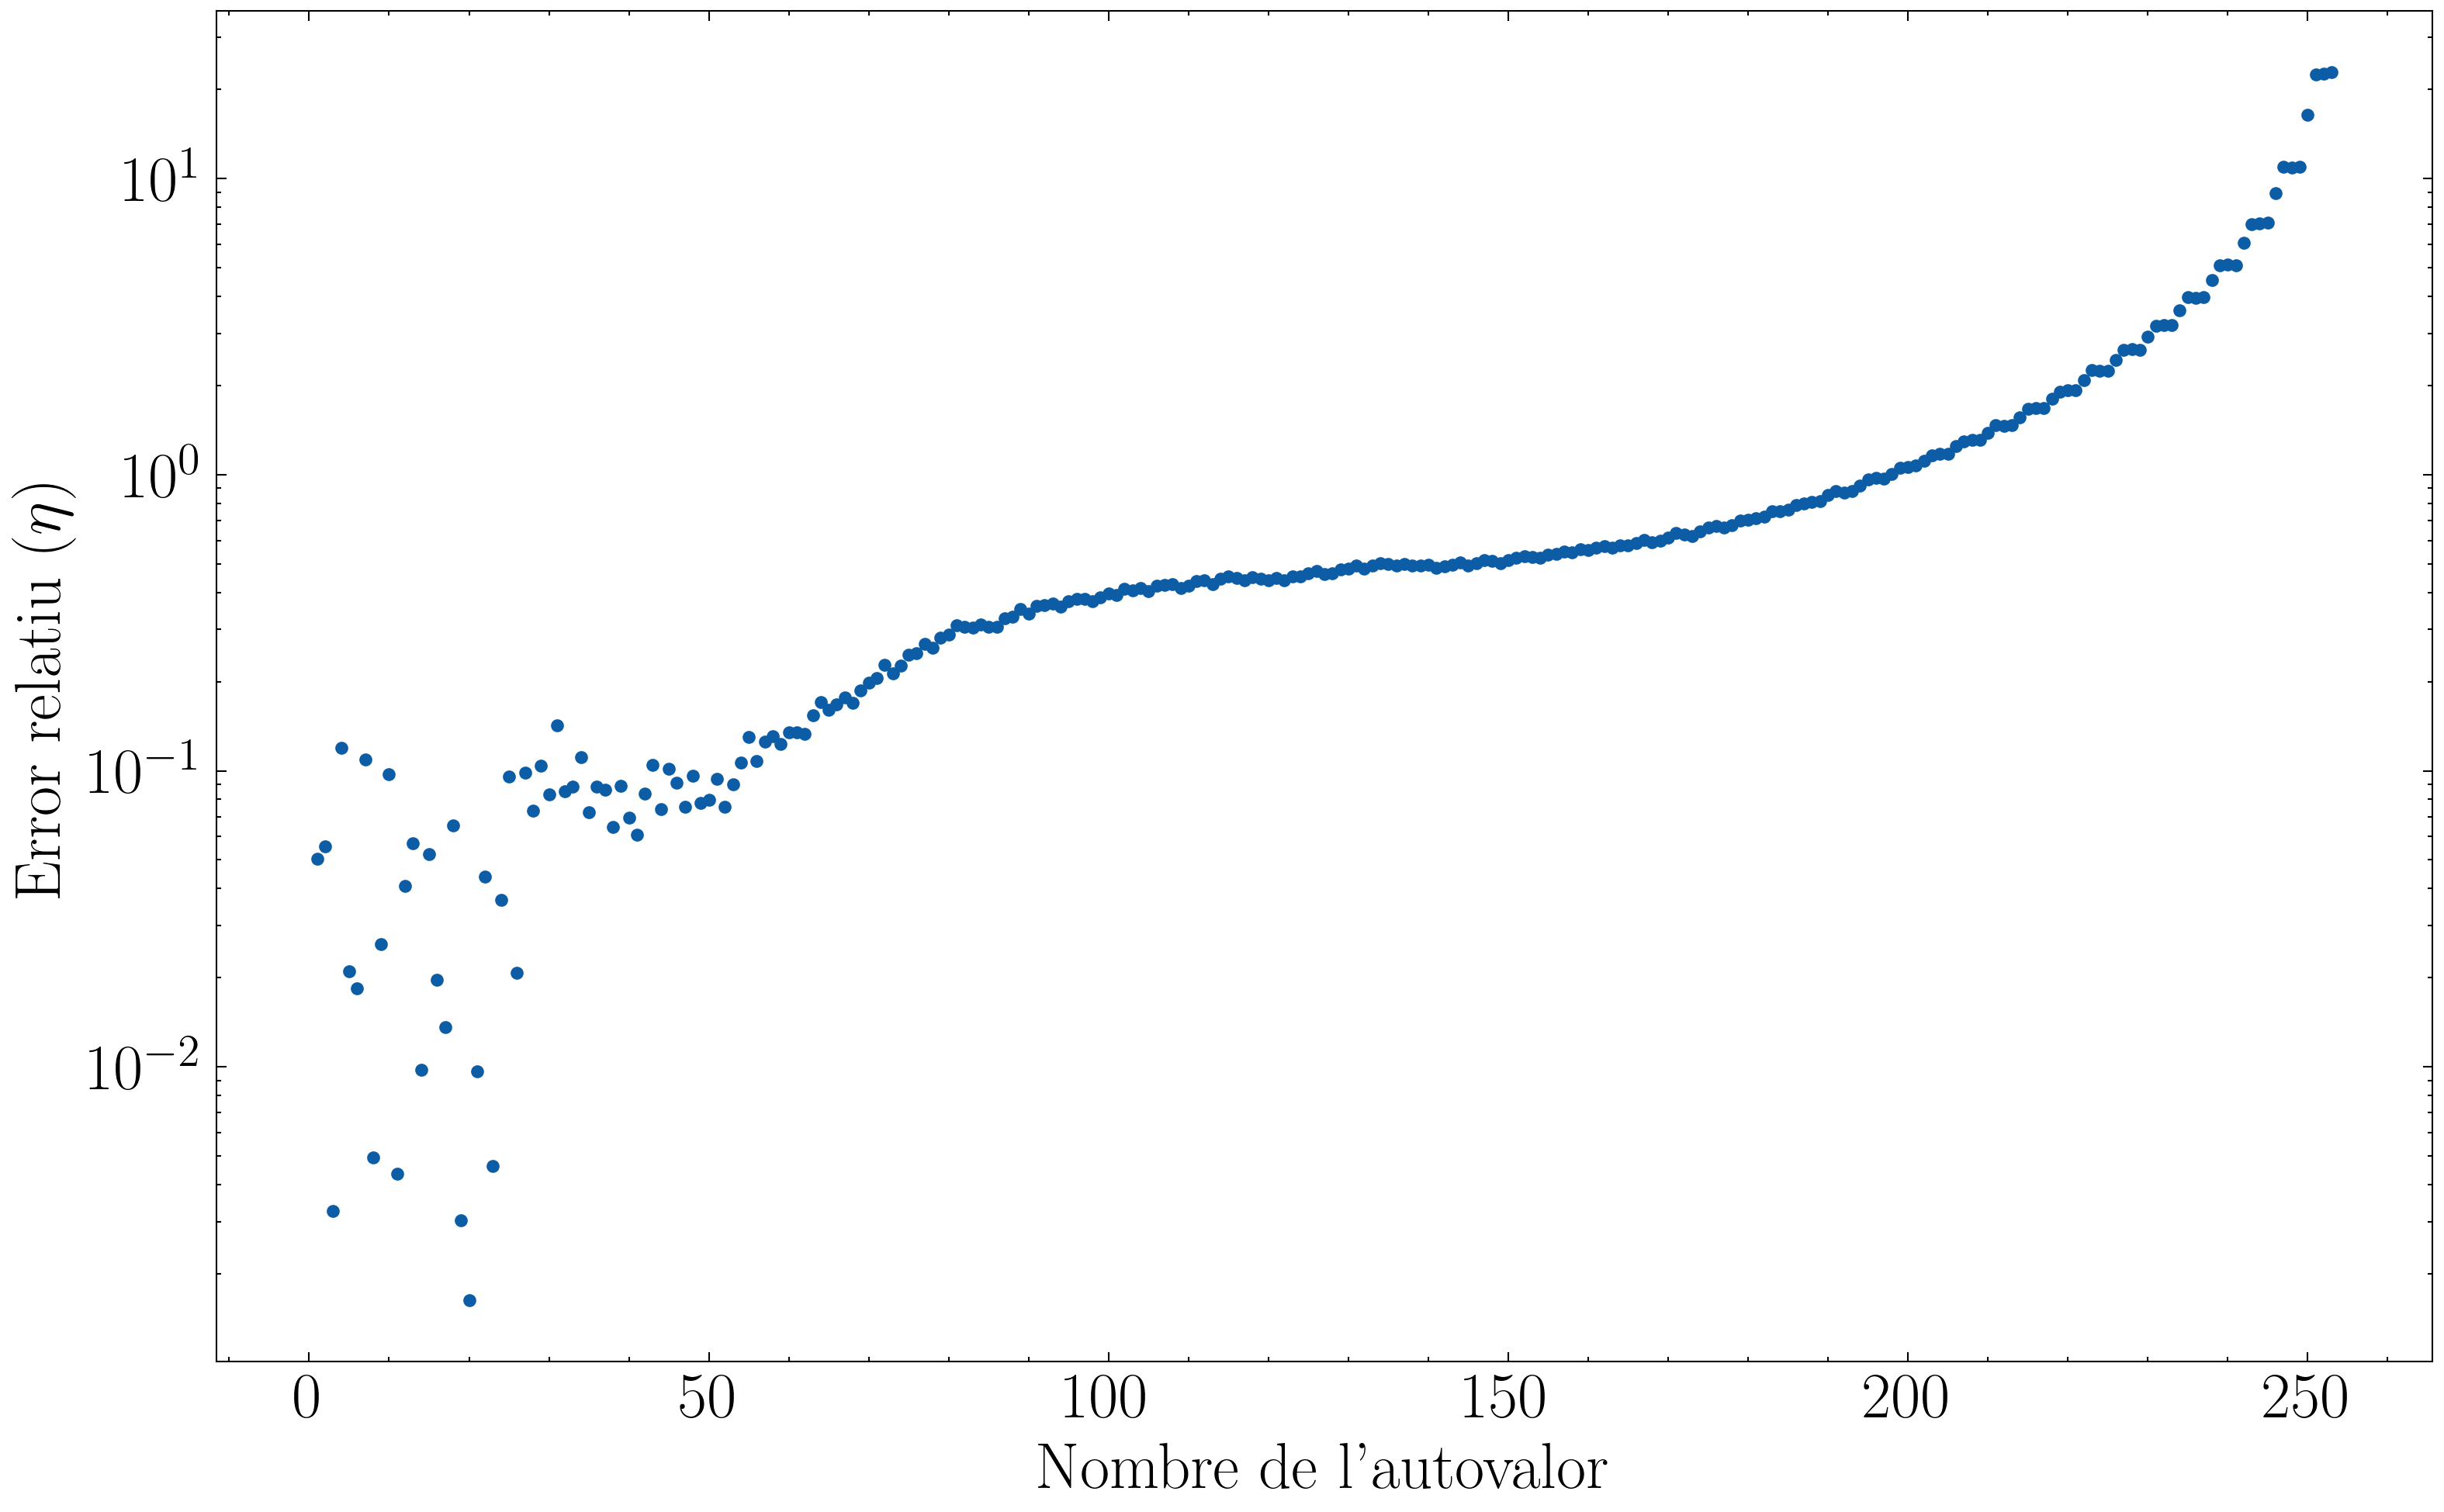
\includegraphics[width=0.95\textwidth]{Figures_Alfven_modes/eigenvalue_error_vA.png}
	\caption{Error relatiu dels autovalors analítics i els calculats amb Dedalus en el cas del problema d'Alfvén.}
	\label{fig:error_vA}
\end{figure}
\vspace{-10pt}


Les autofuncions dels modes d'Alfvén són idèntiques a les d'una corda amb estructura longitudinal.
Per consegüent, l'estructura que segueixen ve determinada pel seu índex de~mode.
El primer és el fonamental, f, el segon és el primer harmònic, 1h, etc.%el tercer 2h, etc.
%El primer és el fonamental, f, el segon és el primer harmònic, 1h, el tercer és el segon harmònic, 2h,
%i així successivament, com es pot observar a la figura següent.
\begin{figure}[H]
	\centering
	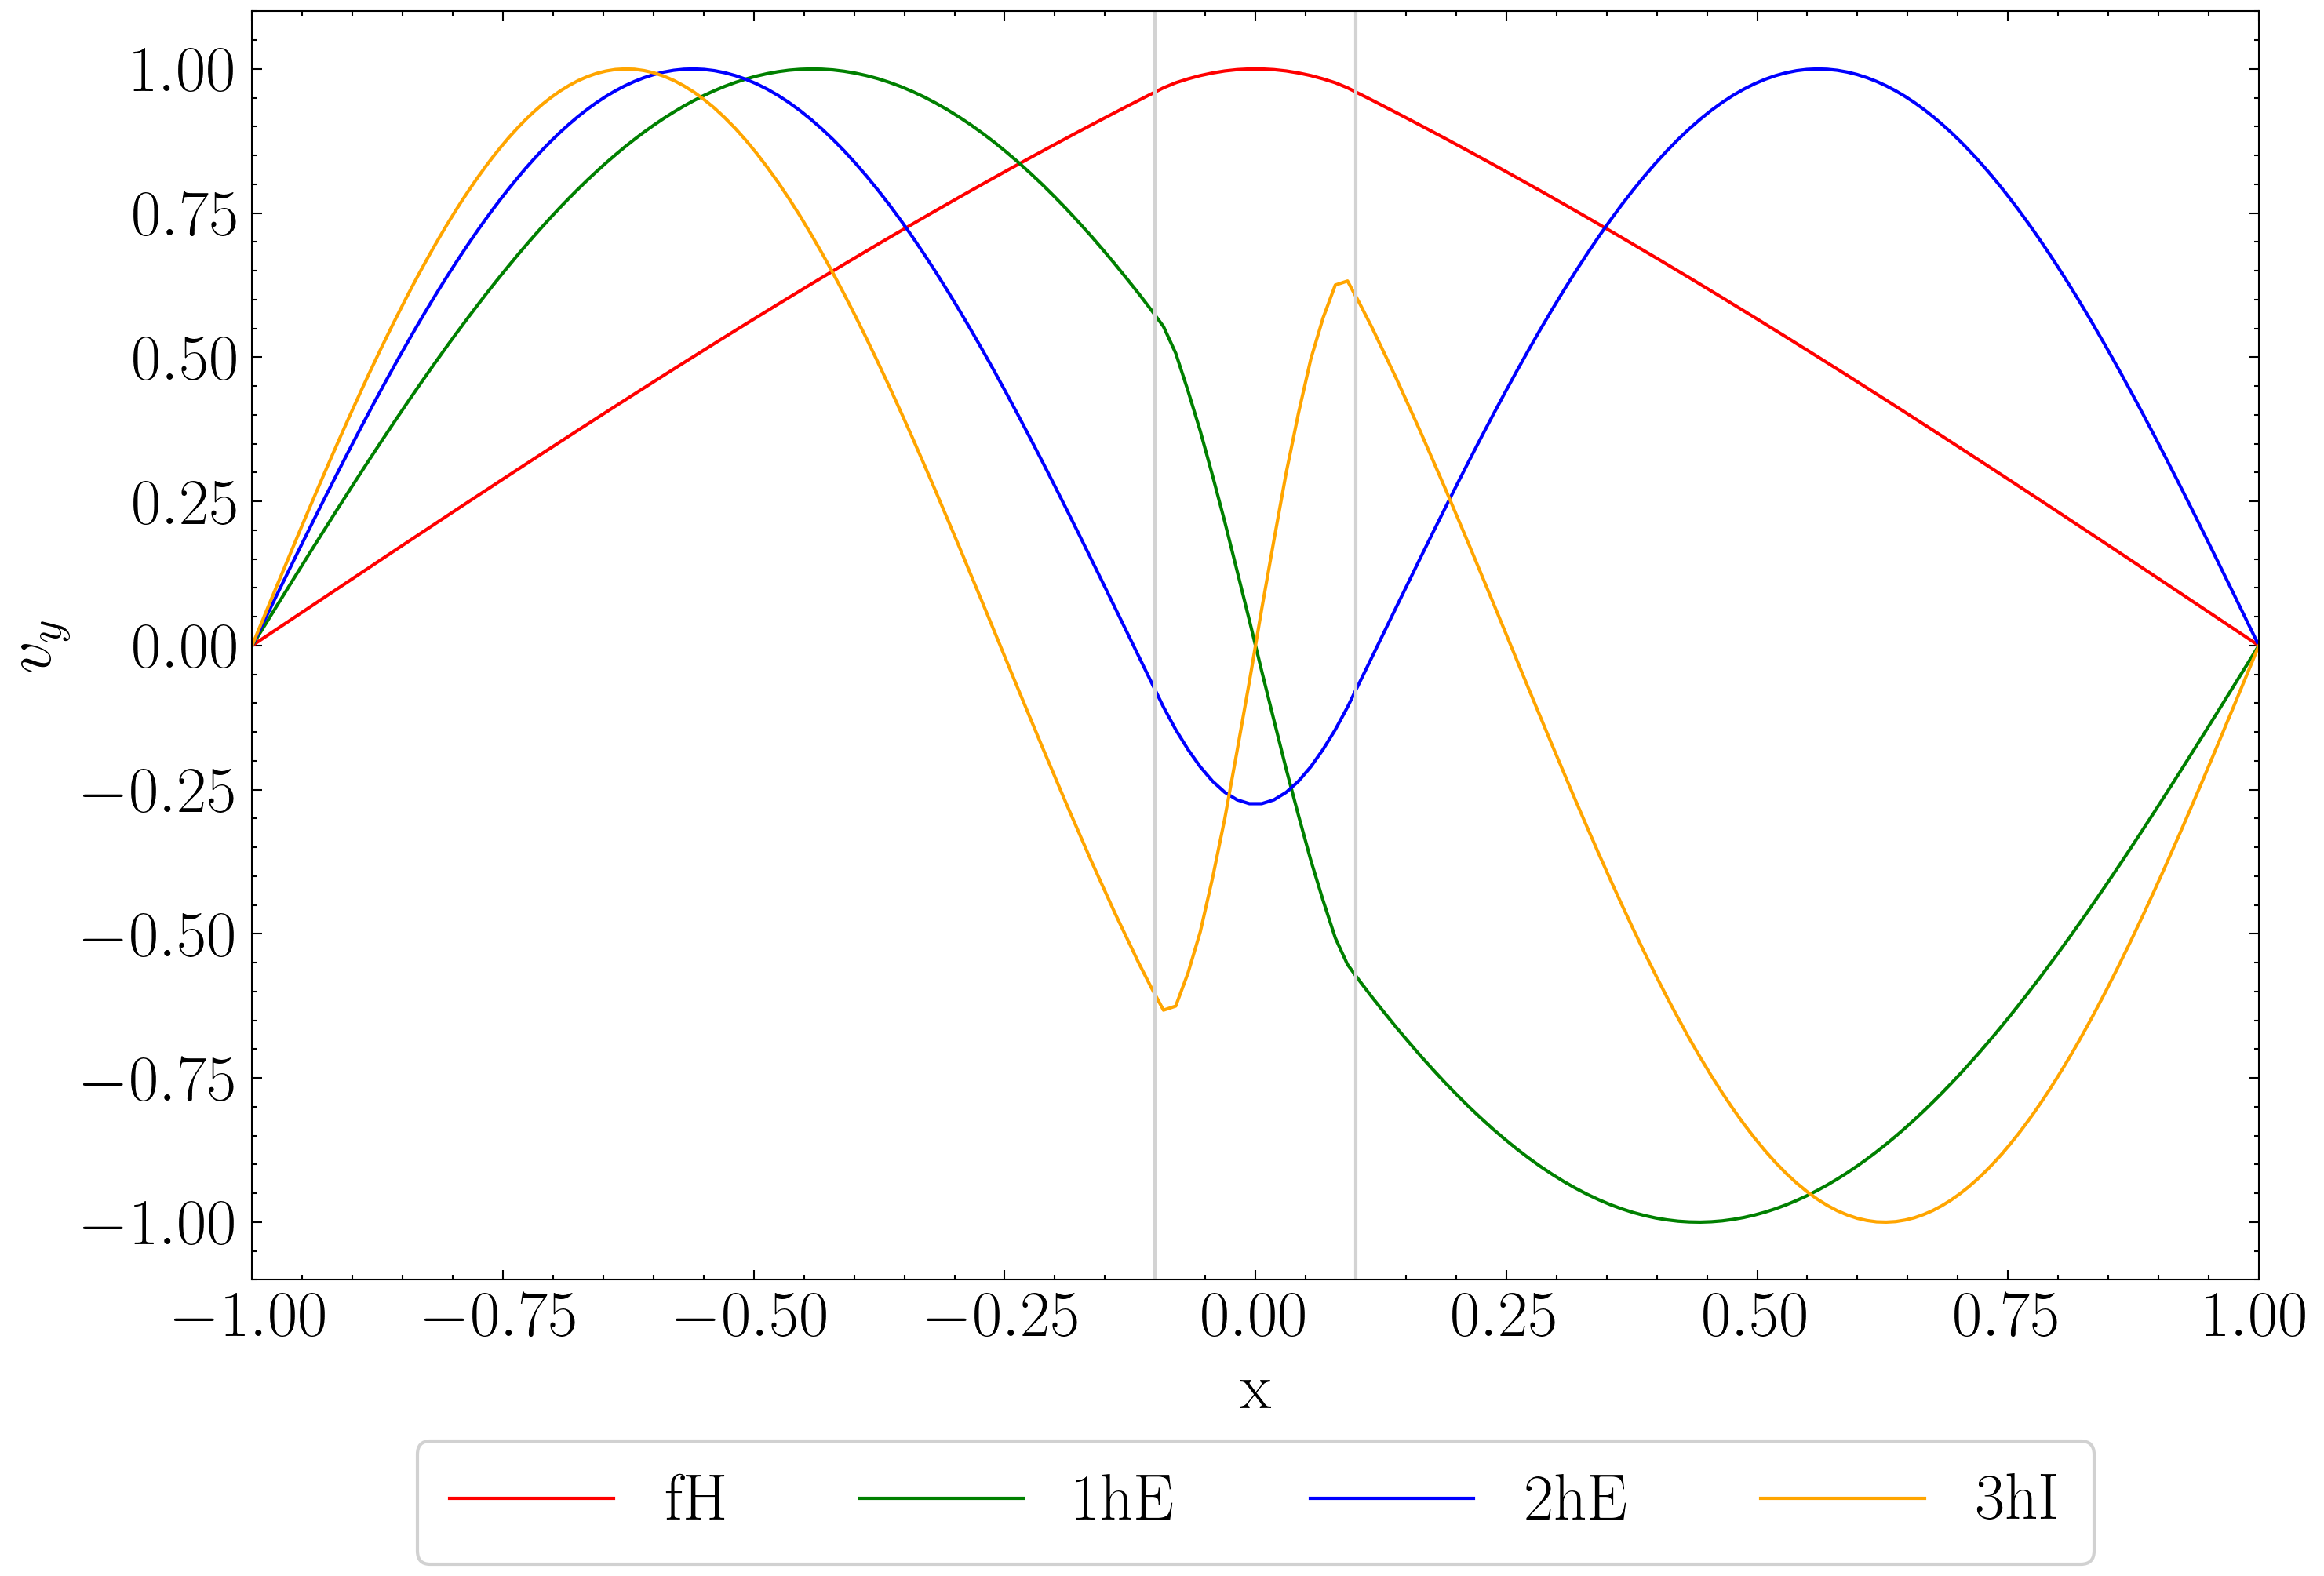
\includegraphics[width=0.95\textwidth]{Figures_Alfven_modes/modes_Alfven.png}
	\caption{Estructura de les primeres autofuncions dels modes d'Alfvén.}
	\label{fig:modes_vA}
\end{figure}
\vspace{-10pt}
Les autofuncions estan fortament condicionades per les diferències en la velocitat d'Alfvén, apart de la consideració dels extrems fixes.
Aquesta velocitat és molt major en l'interior, la prominència, que en l'exterior, la corona,
de manera que la variació en velocitat dels modes en la protuberància és major.

%Com ja s'ha esmentat, per advertir el comportament extern, intern o híbrid dels modes s'ha fet servir el quadern de Mathematica, veure apèndix~[\ref{ap.A}].

Les parts imaginàries de les autofuncions són nul·les i no es presenten gràficament.
La informació rellevant és continguda en la part real.
En el càlcul numèric no són estrictament zero degut a la limitació de 16 decimals de Python,
tot i que són de l'ordre de $10^{-13}$ respecte a la part real normalitzada.



\section{Modes ràpids i lents} \label{subsec:resultats_modes_r_i_l}
En aquest cas és convenient començar per la representació de la relació de dispersió de l'Eq.~(\ref{eq.3.34}).
És a dir, l'evolució dels autovalors, $\omega$, segons la constant d'acoblament, $\bm{k}$.
D'acord amb les Eqs.~(\ref{eq.3.32}) i (\ref{eq.3.33}) l'única direcció del vector d'ona que acobla els modes és la paral·lela a la protuberància, $k_z$.
\begin{figure}[H]
	\centering
	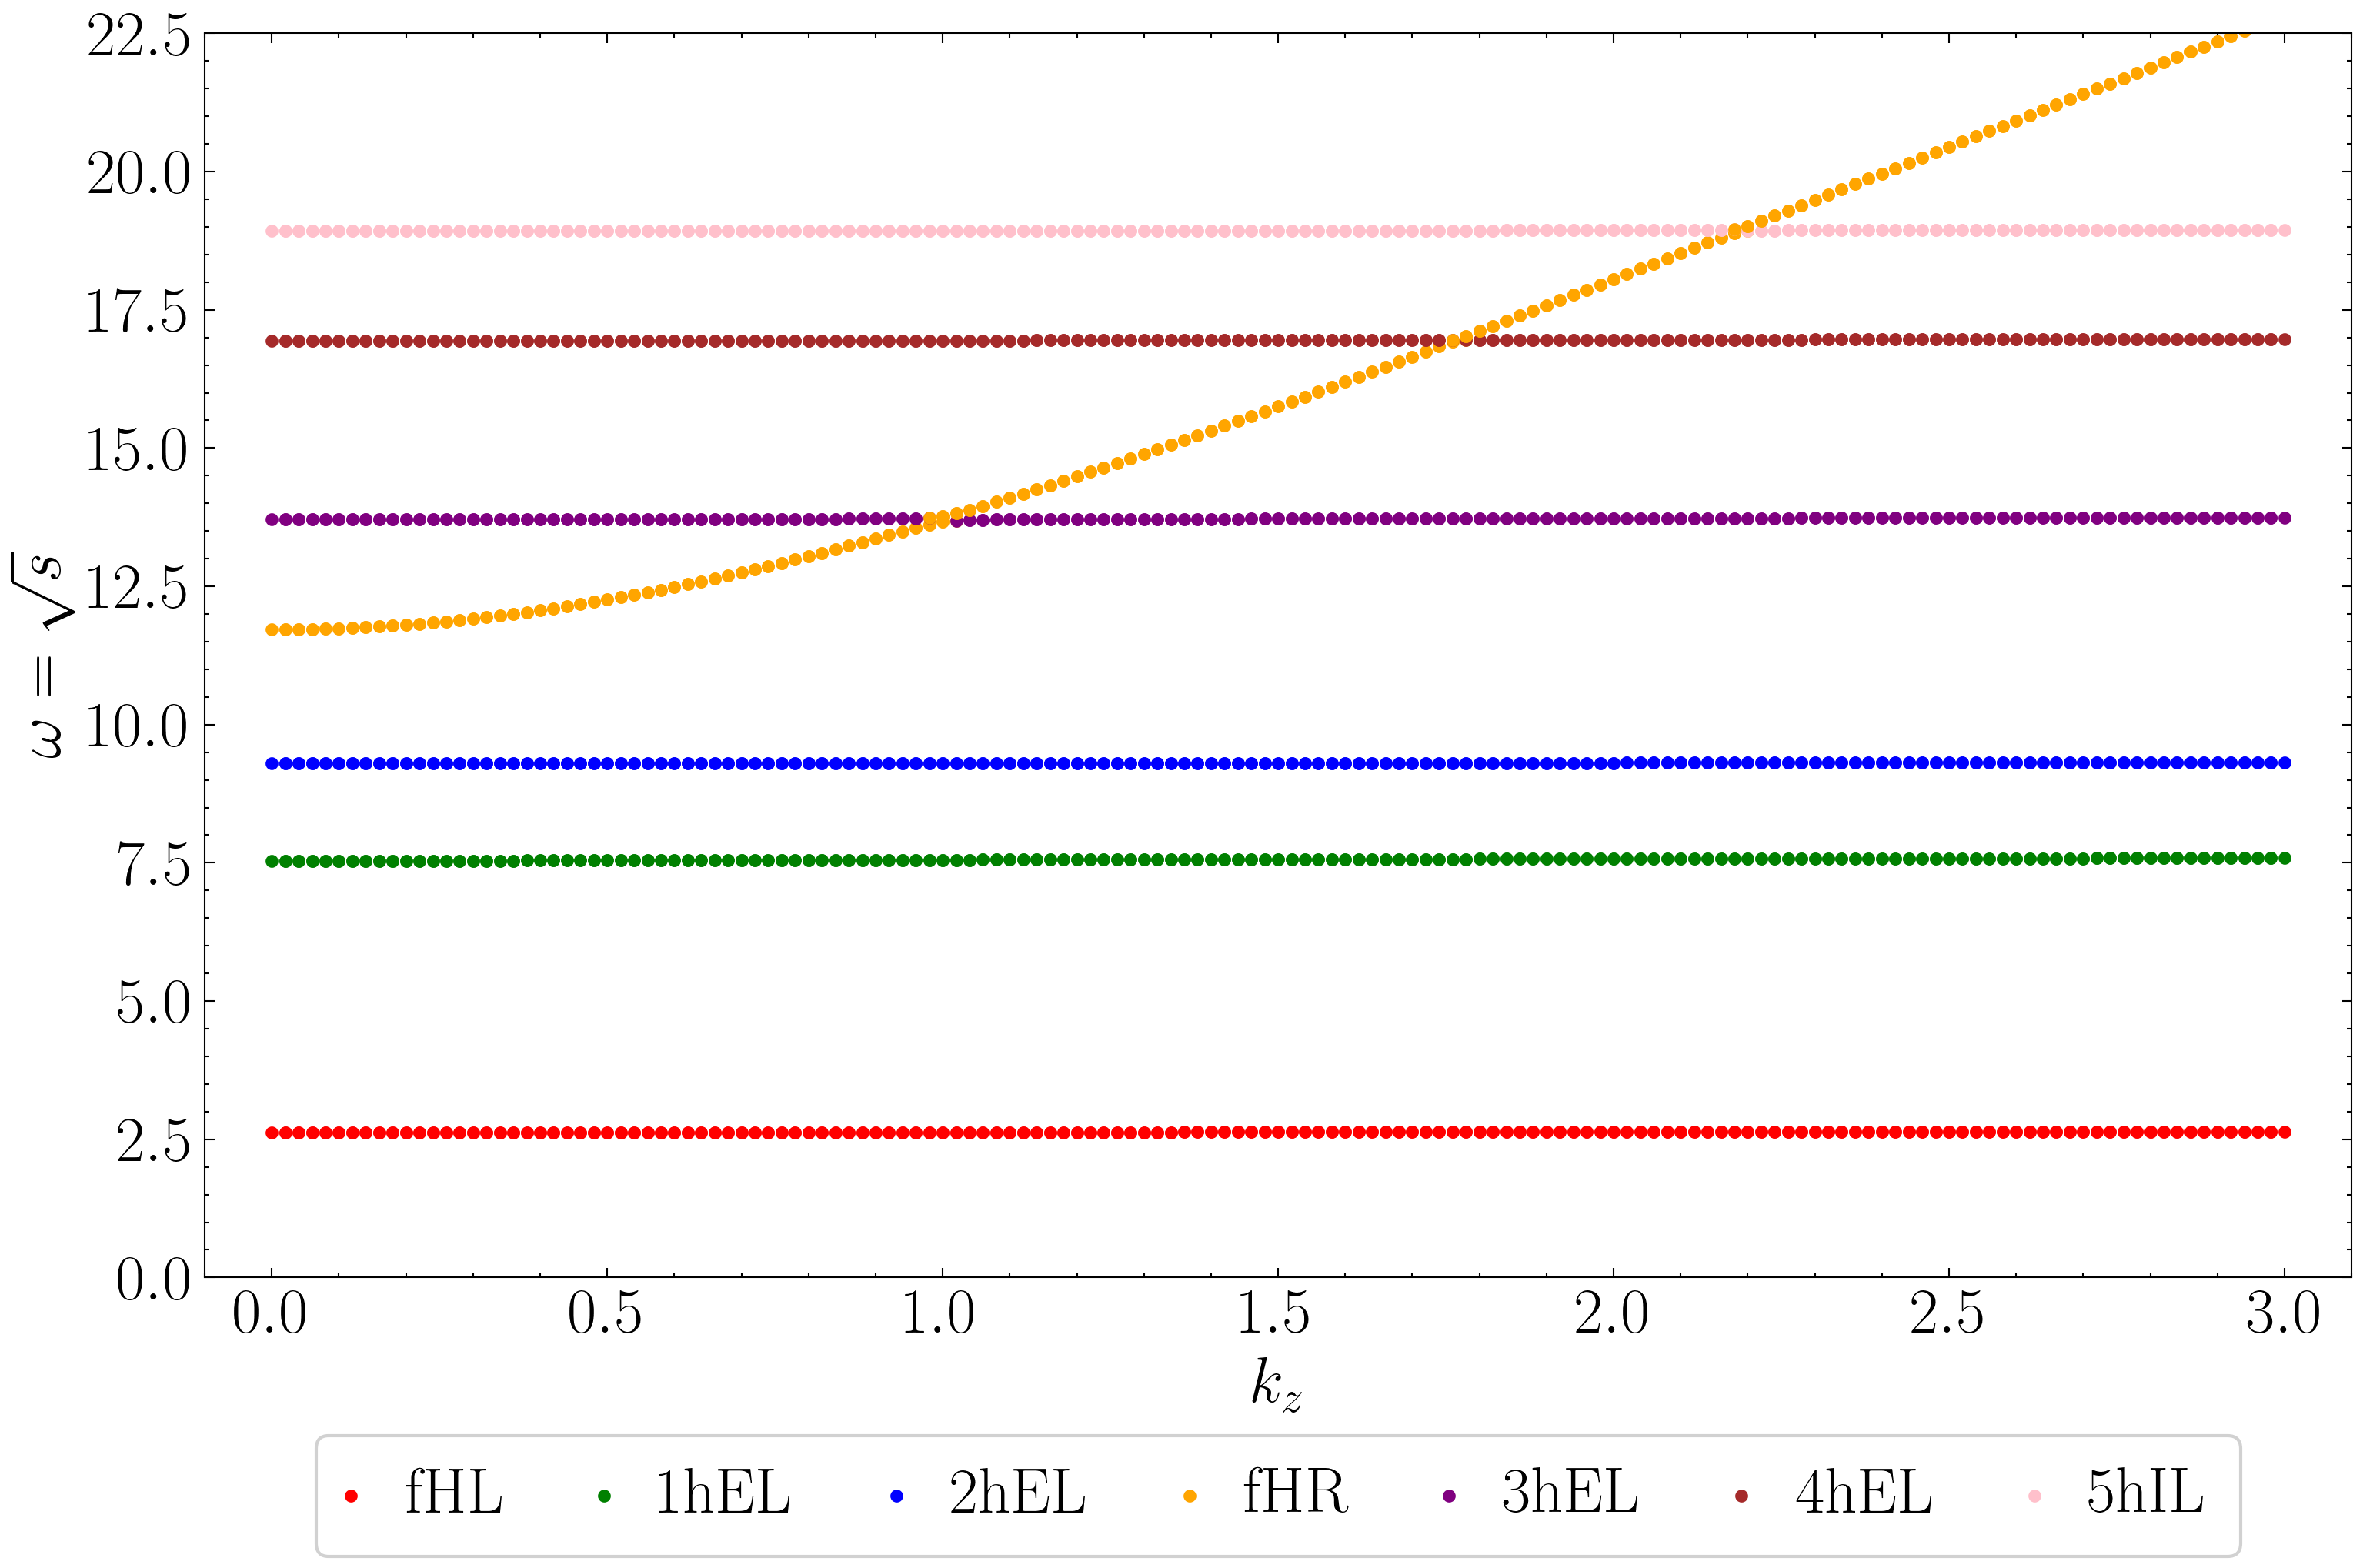
\includegraphics[width=0.95\textwidth]{Figures_F&S_modes/dd_modes_normals.png}
	\caption{Diagrama de dispersió.}
	\label{fig:dd}
\end{figure}
\vspace{-10pt}
De nou, les etiquetes corresponen a l'explicació anterior.
Tanmateix en aquest cas s'afegeix la tercera per indicar si el mode és ràpid, R, ò lent, L, d'acord amb l'article de \textcite{oscillation_modes_II}.
Aquesta qualitat s'aprecia directament amb l'evolució dels modes: els modes ràpids són parabòl·lics i els modes lents sóns constants.
Cada color i etiqueta del diagrama de dispersió de la Fig.~\ref{fig:dd} correspon a un mode del problema.
Aquests són analitzats més envant en el treball i es representen les seves autofuncions amb els colors i eteiquetes que els pertoquen.

%---------------------------------------------------------------------------------------------------------------------------------------------------
% Es pot citar i/o mencionar una figura/secció que encara no ha aparegut?
%---------------------------------------------------------------------------------------------------------------------------------------------------


Els modes normals calculats no corresponen directament als modes ràpids i lents.
Cada mode normal s'etiqueta en $k_z = 0$ partint del $n = 1$, en vermell, fins al $n = 7$, en rosa.
Aquests s'han de treballar per arribar als modes ràpids i lents.

Per entendre bé la situació es representa l'evolució del mode normal amb $n = 5$, inicialment de color morat, i s'analitzen els seus canvis de creixement.
S'ha escollit aquest mode atès que aquest presenta dos canvis de tendència, així com $n = 6$, de primeres representat en color grana. En qualsevol cas,
el cinquè mode normal apareix en el primer intercanvi de comportament, aprop de $k_z \sim 1$, que més envant s'estudia aquest cas en detall.
La situació d'intercanvi de comportament dels modes normals es defineix en l'article d'\textcite{oscillations_quiescent_solar_prominence}
com un ``encreuament evitat''.

Els modes d'ordre superior no es mostren en figures posteriors per qüestions visuals,
encara que s'han treballat per conéixer la seva naturalesa, expressada en les etiquetes.
\begin{figure}[H]
	\centering
	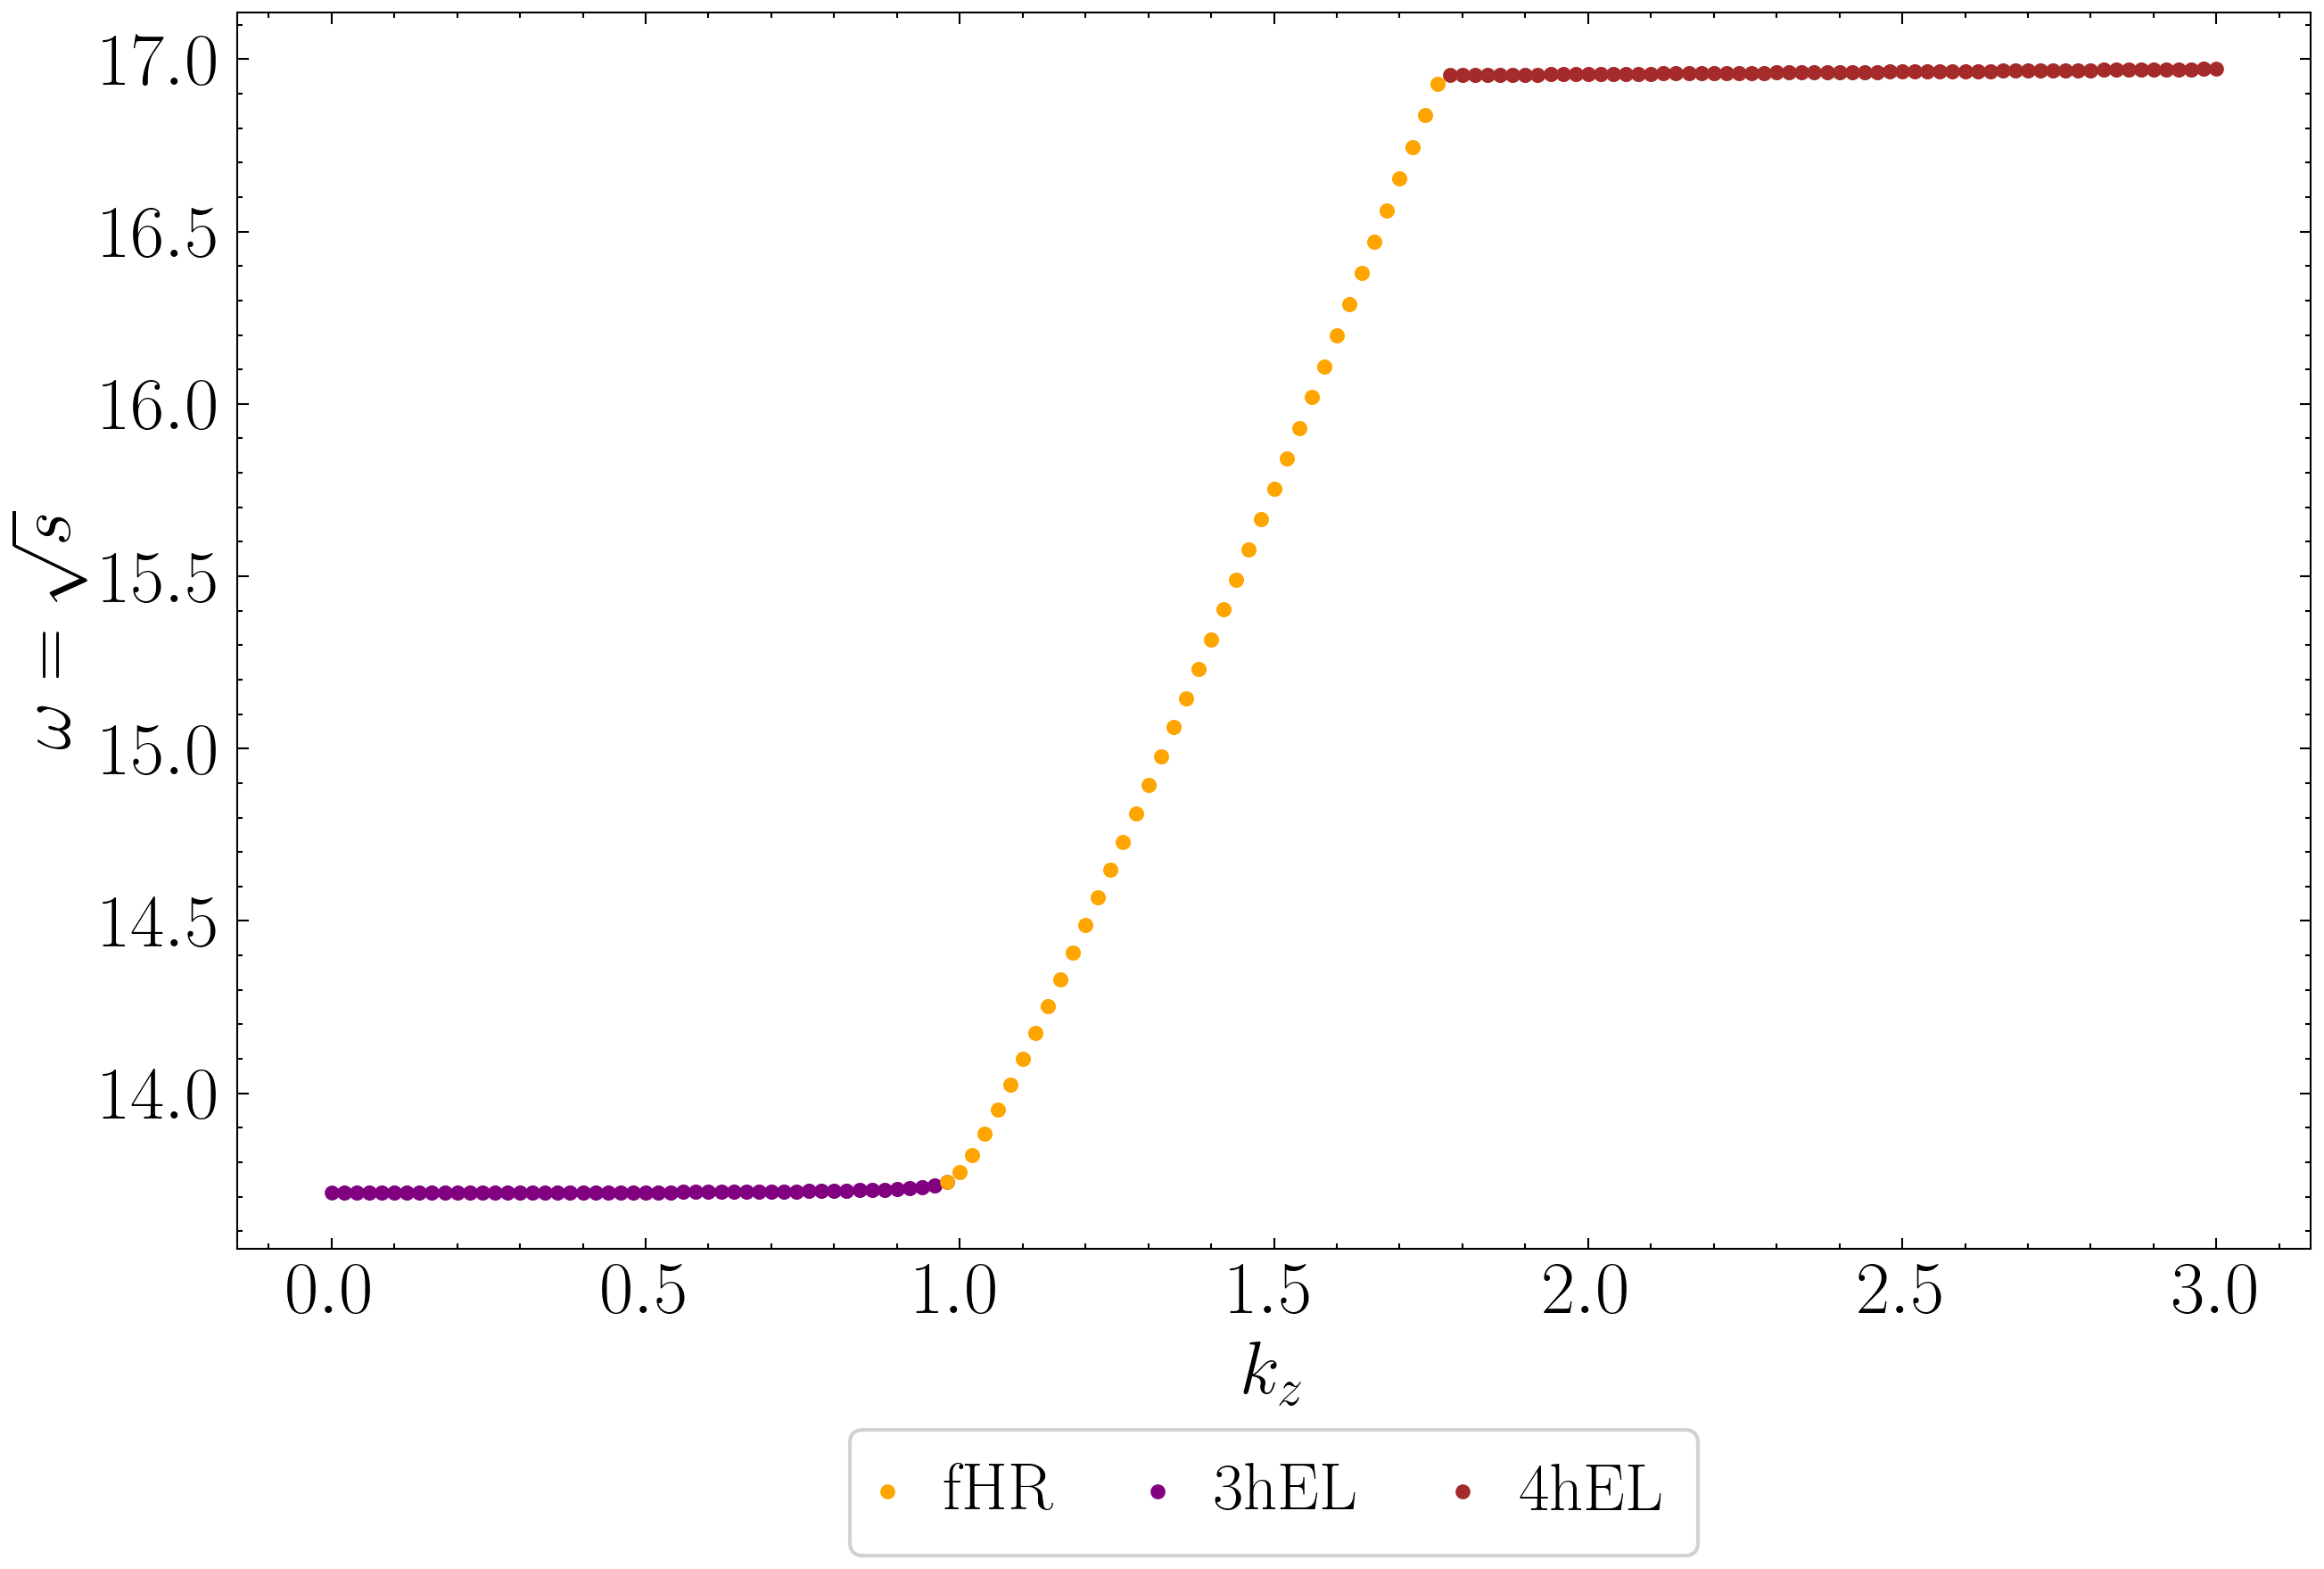
\includegraphics[width=0.95\textwidth]{Figures_F&S_modes/dd_mode_5.png}
	\caption{Evolució d'un mode normal individual (n = 5).}
	\label{fig:dd_mode_5}
\end{figure}
\vspace{-10pt}
Inicialment aquest mode és lent (3hFL) però aprop de $k_z \sim 1$ hi ha una inversió del comportament i passa a ser ràpid.
El creixement sobtat de l'autovalor ho determina, a diferència de la invariància d'aquest en el mode lent, en $k_z < 1$.
Envoltant de $k_z \sim 1.8$ es desfà el canvi i es recupera el mode lent (4hEL),
ara bé, és un mode lent harmònic d'un ordre superior a l'inicial.
%Aquests fets es comproven més envant dins aquesta secció amb l'estudi de les autofuncions. 

L'evolució del mode normal $n = 5$ no s'entèn si es mira de manera aïllada.
Per comprendre la situació s'ha de recuperar la Fig.~\ref{fig:dd} i s'ha d'apreciar que el mode normal anterior, $n = 4$,
és inicialment un mode ràpid, amb un creixement parabòl·lic, fins a $k_z \sim 1$.
És en aquest punt on es realitza un encreuament evitat amb el mode superior degut a que aquests no poden solapar-se, de manera que cerquen camins diferents.

Amb el fi d'observar el canvi de conducta dels modes s'amplia el diagrama de dispersió de la Fig.~\ref{fig:dd} aprop del canvi, en $k_z \sim 1$.
\begin{figure}[H]
	\centering
	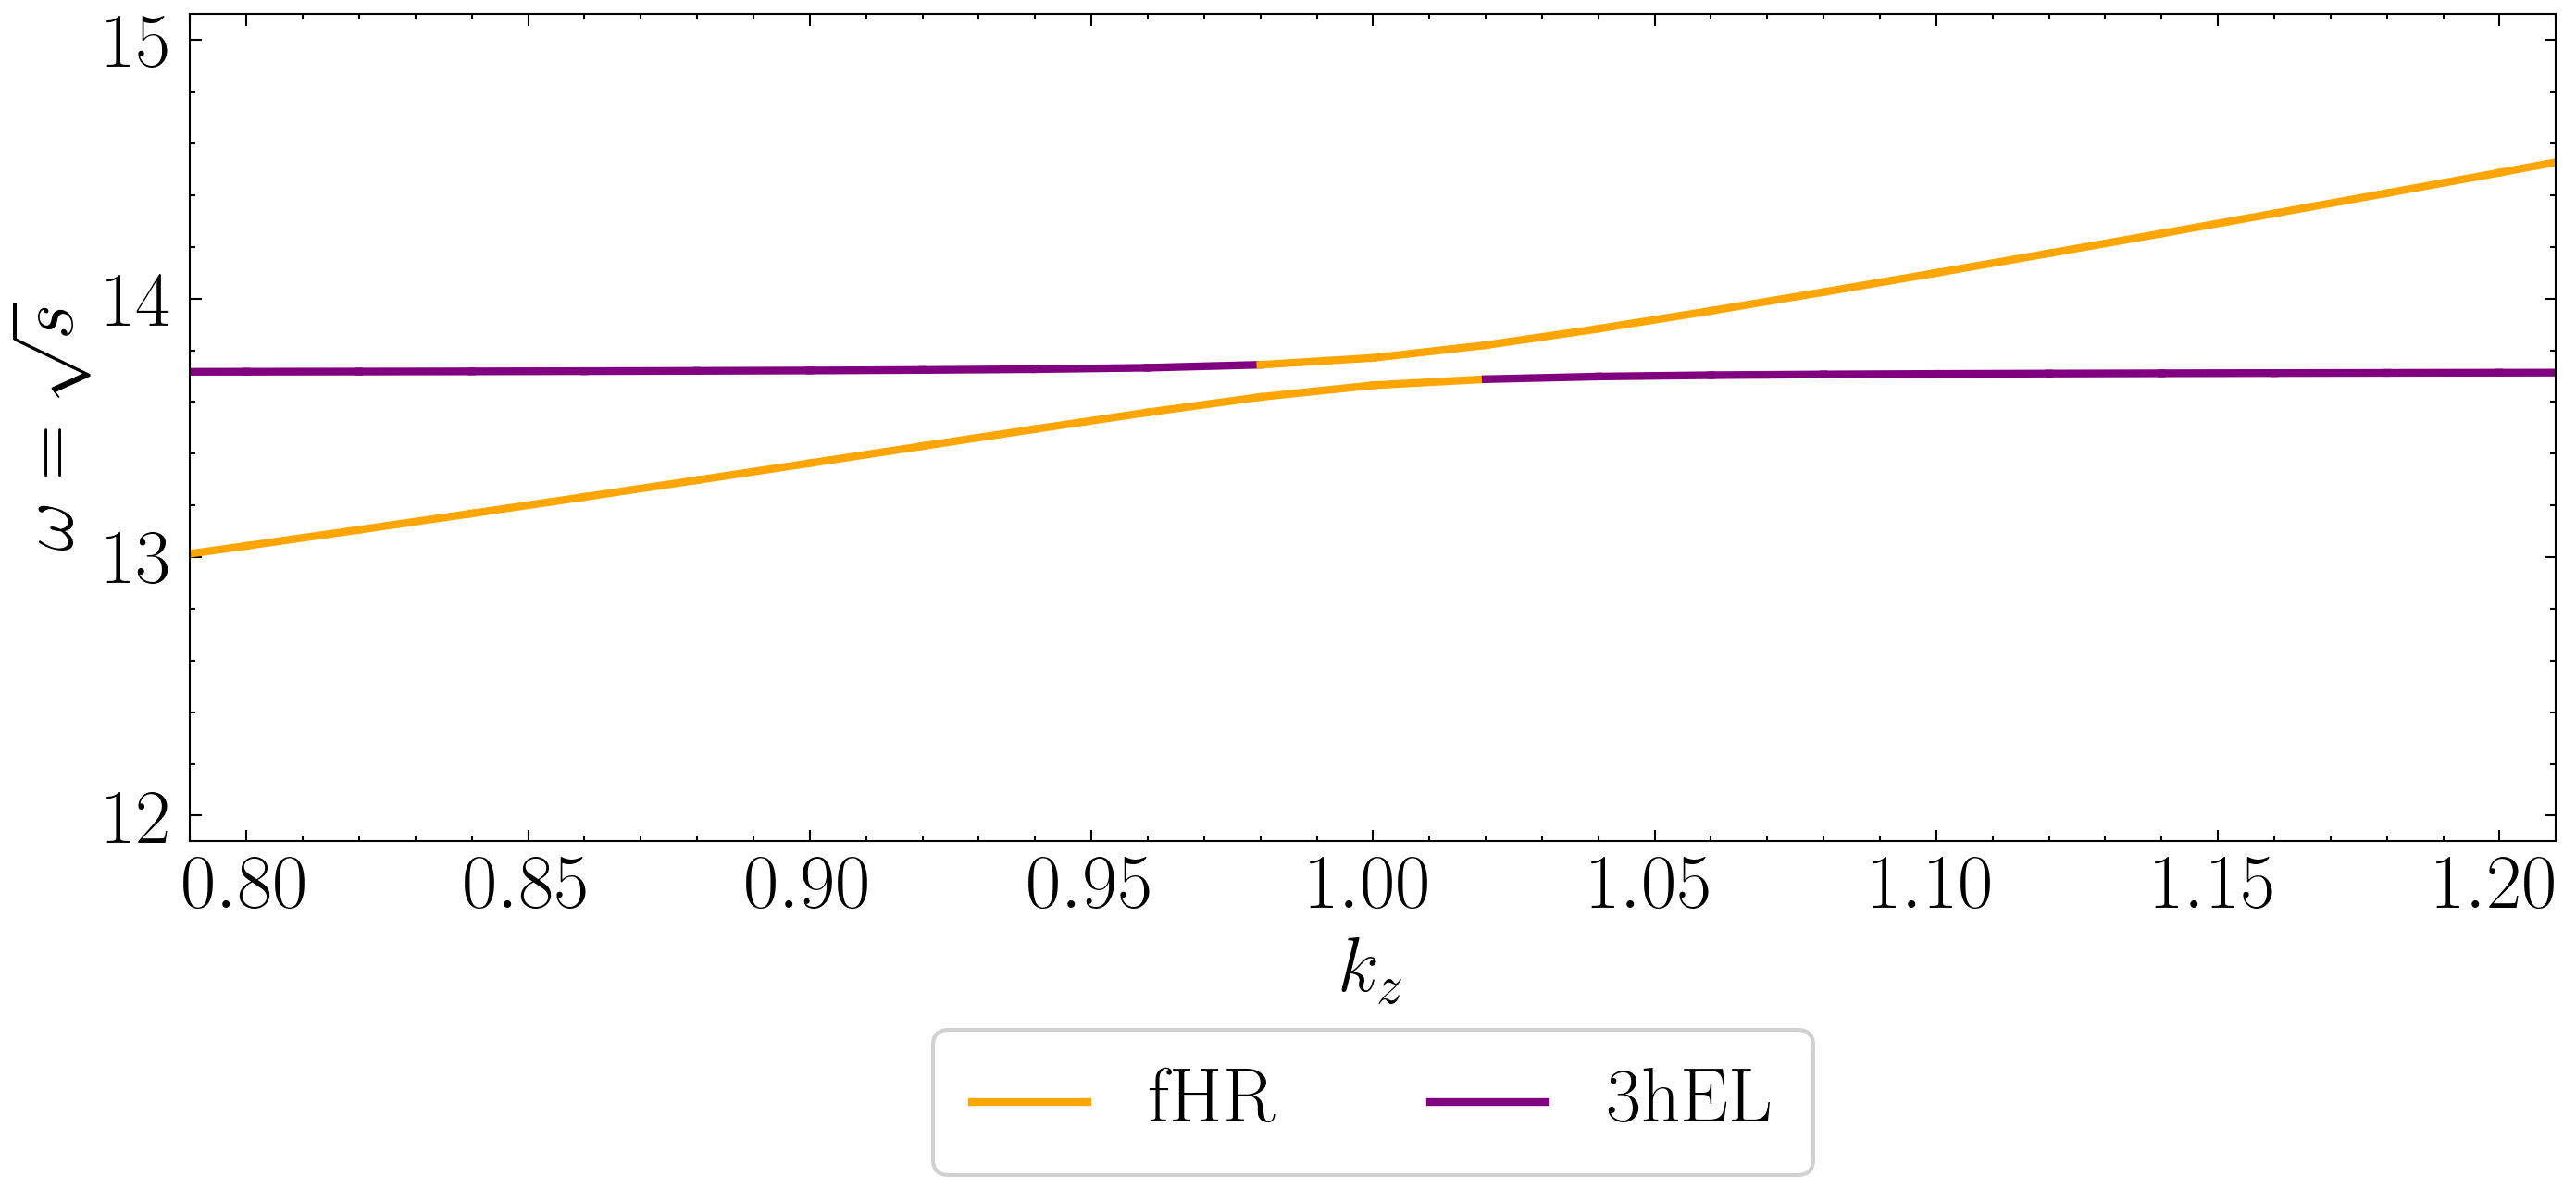
\includegraphics[width=0.95\textwidth]{Figures_F&S_modes/first_anticrossing.png}
	\caption{Encreuament evitat entre els modes fHR i 3hEL.}
	\label{fig:dd_avoided_crossing}
\end{figure}
\vspace{-10pt}
En aquest cas s'interpolen linealment els punts de la relació de dispersió per demostrar explícitament que es tracta d'un encreuament evitat.
Així, és evident que els modes en sí no es creuen i que hi ha un intercanvi de tendència d'aquests, així com s'havia explicat anteriorment.

%---------------------------------------------------------------------------------------------------------------------------------------------------
%Vz va en direcció del camp i no li afecta molt l'acoblament de kz --- afegir al tfg --- a quina secció? teoria? i despres s'observa en l'evolució del mode fHR --- sí!

%La velocitat paral·lela a la direcció d'acoblament, $v_z$, no es veu molt alterada per l'acoblament precisament.
%Aquest fet és un reflexe de les equacions dels modes ràpids i lents, Eqs.~(\ref{eq.3.32}) i (\ref{eq.3.33})
%---------------------------------------------------------------------------------------------------------------------------------------------------

%\subsubsection{Autofuncions per $k_z$ fixa.}
\subsubsection{Autofuncions amb constant d'acoblament, $k_z$, fixa} \label{subsubsec:kz_constant}

Una vegada estudiat el diagrama de dispersió es representen les autofuncions, és a dir, l'estructura dels modes al llarg de l'eix $\hat{x}$.

Per començar, es calcula l'error relatiu per aquest cas.
L'evolució d'aquest en el cas dels modes ràpids i lents és semblant al del cas d'Alfvén de la Fig.~\ref{fig:error_vA}.
Ara bé, no és exactament igual. En aquest cas l'error és petit i anàrquic en els primers 50 autovalors,
s'estabilitza un poc més alluny, als 150, i als 200 es dispara, de nou per qüestions del càlcul computacional.
\begin{figure}[H]
	\centering
	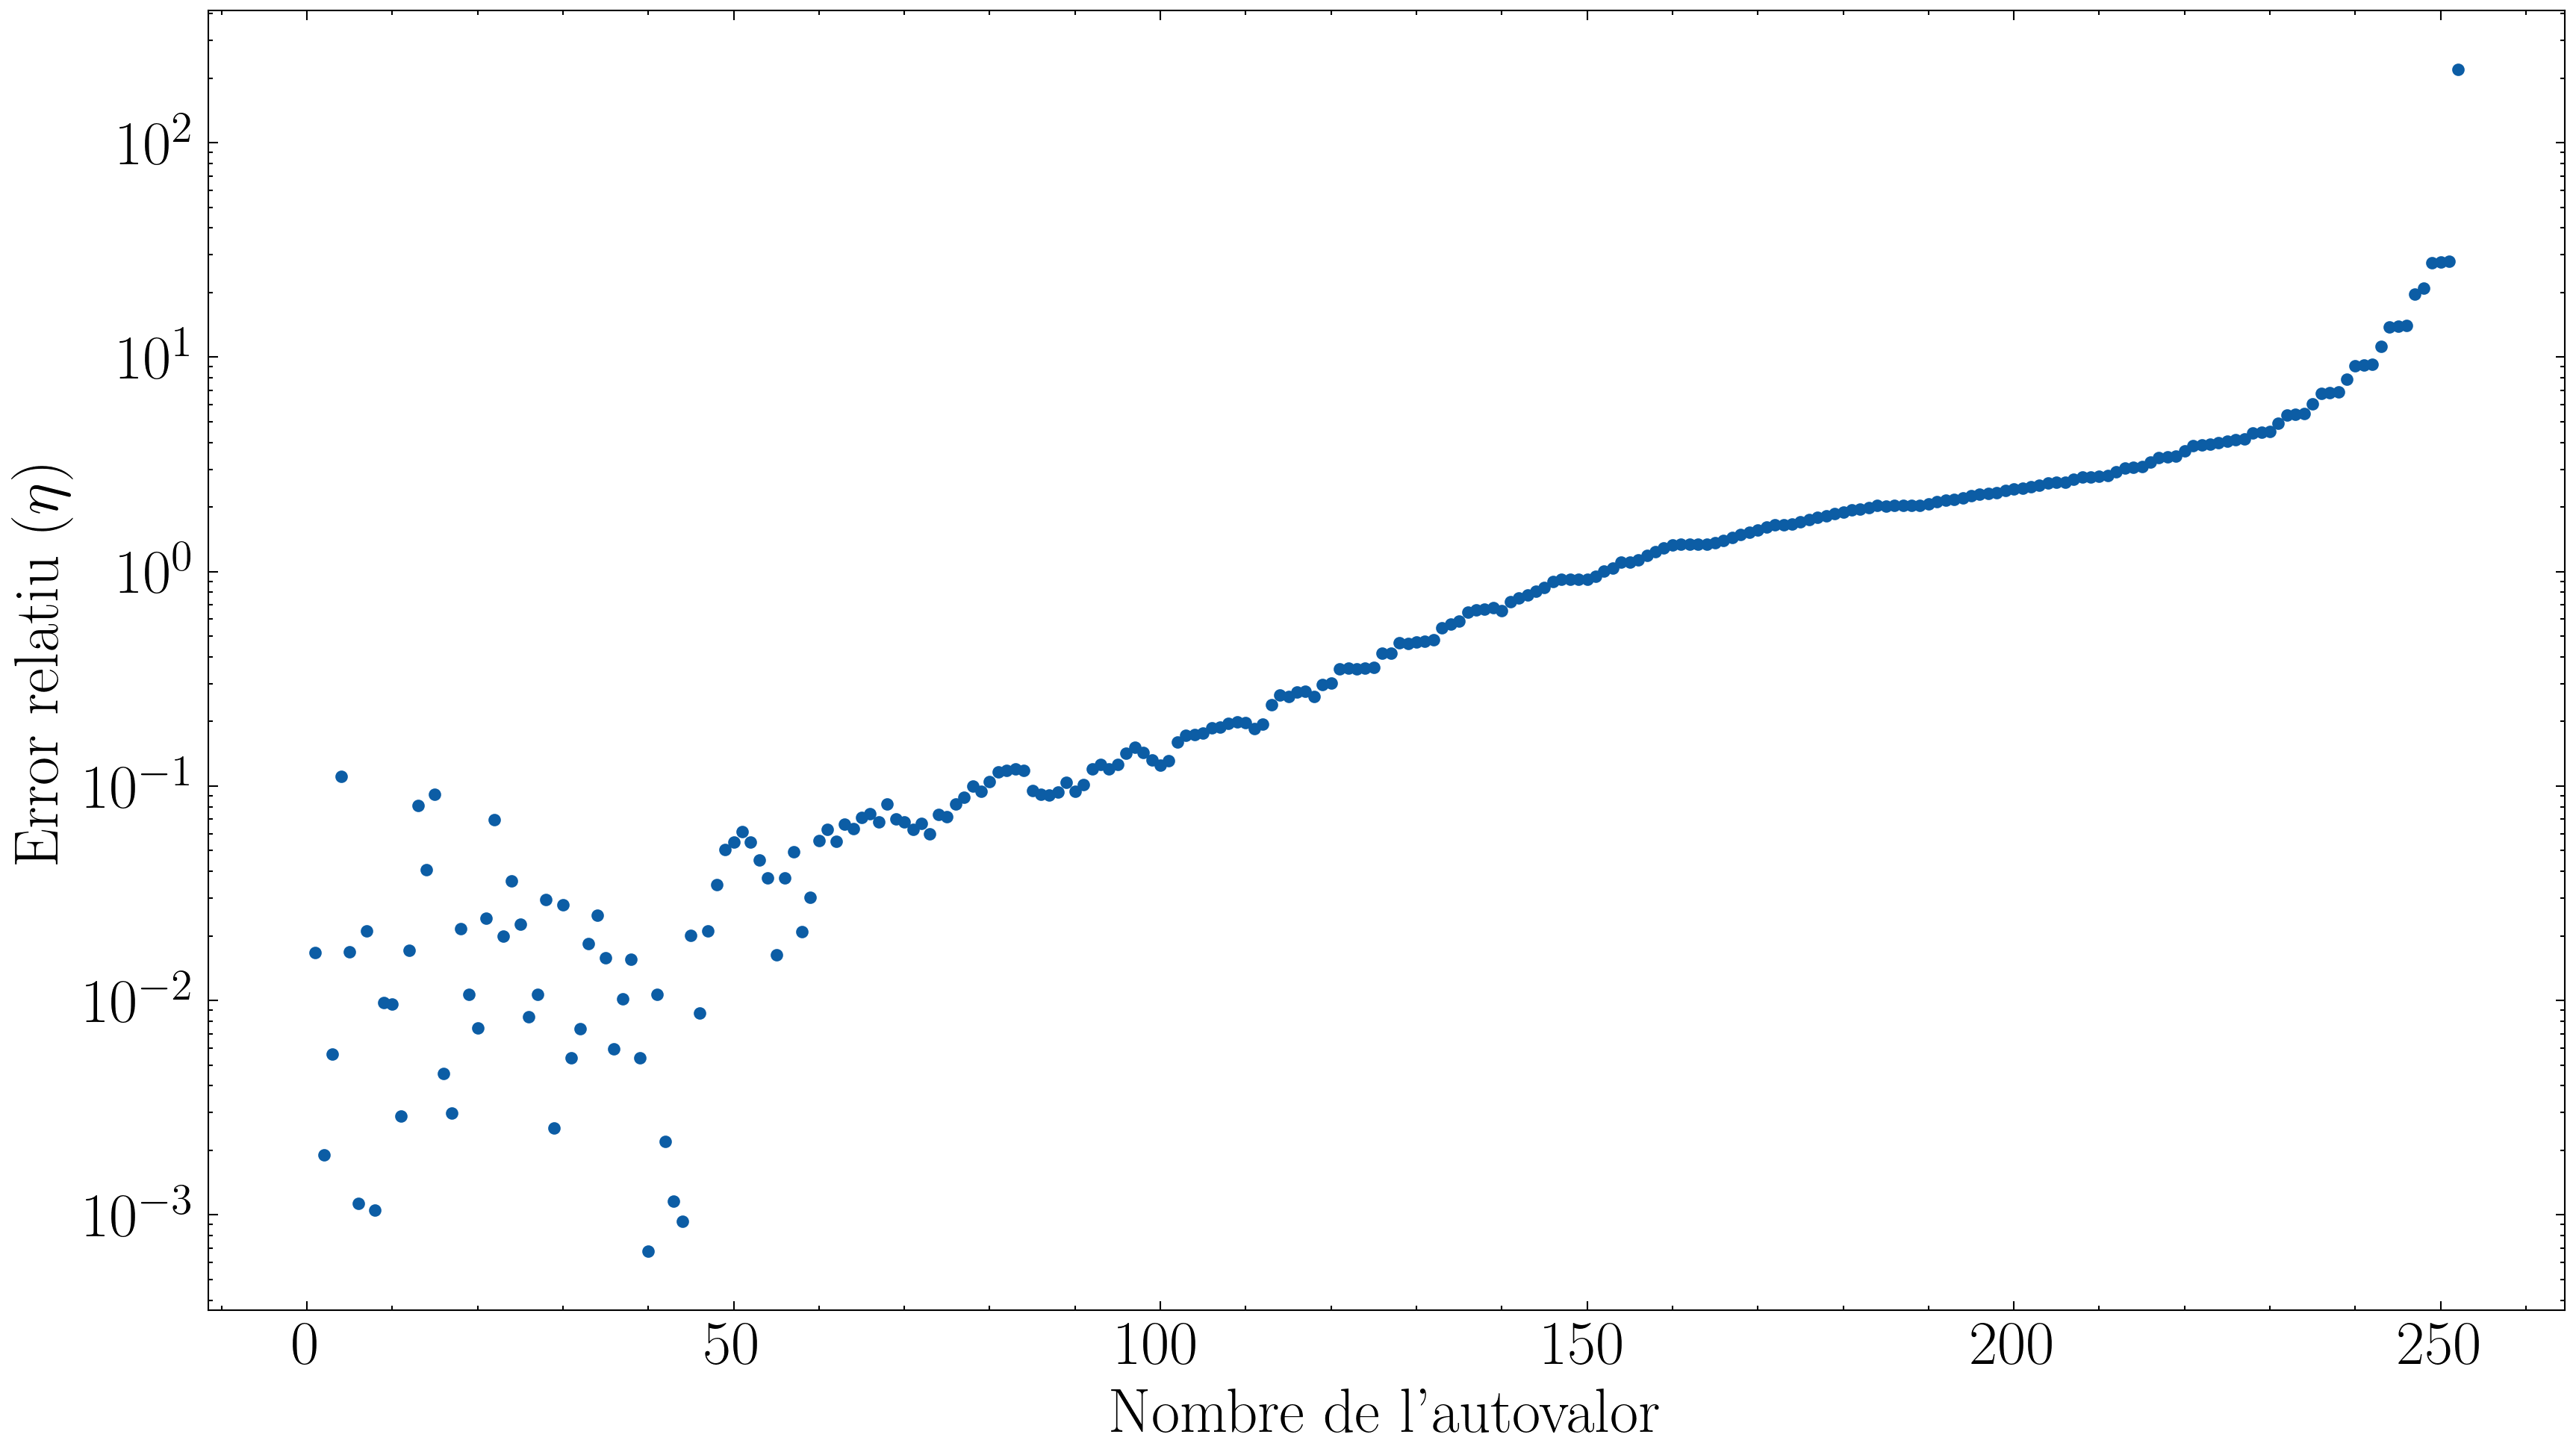
\includegraphics[width=0.95\textwidth]{Figures_F&S_modes/eigenvalue_error.png}
	\caption{Error relatiu dels autovalors analítics i els calculats amb Dedalus en el cas dels modes ràpids i lents.}
	\label{fig:error_relatiu_r_i_l}
\end{figure}
\vspace{-10pt}

Finalment es presenten les autofuncions en sí, l'estructura dels modes.
Es considera una constant d'acoblament petita, $k_z = 0.01$,
per poder apreciar la diferència amb els modes d'Alfvén de la Fig.~\ref{fig:modes_vA} de l'apartat anterior.
\begin{figure}[H]
	\centering
	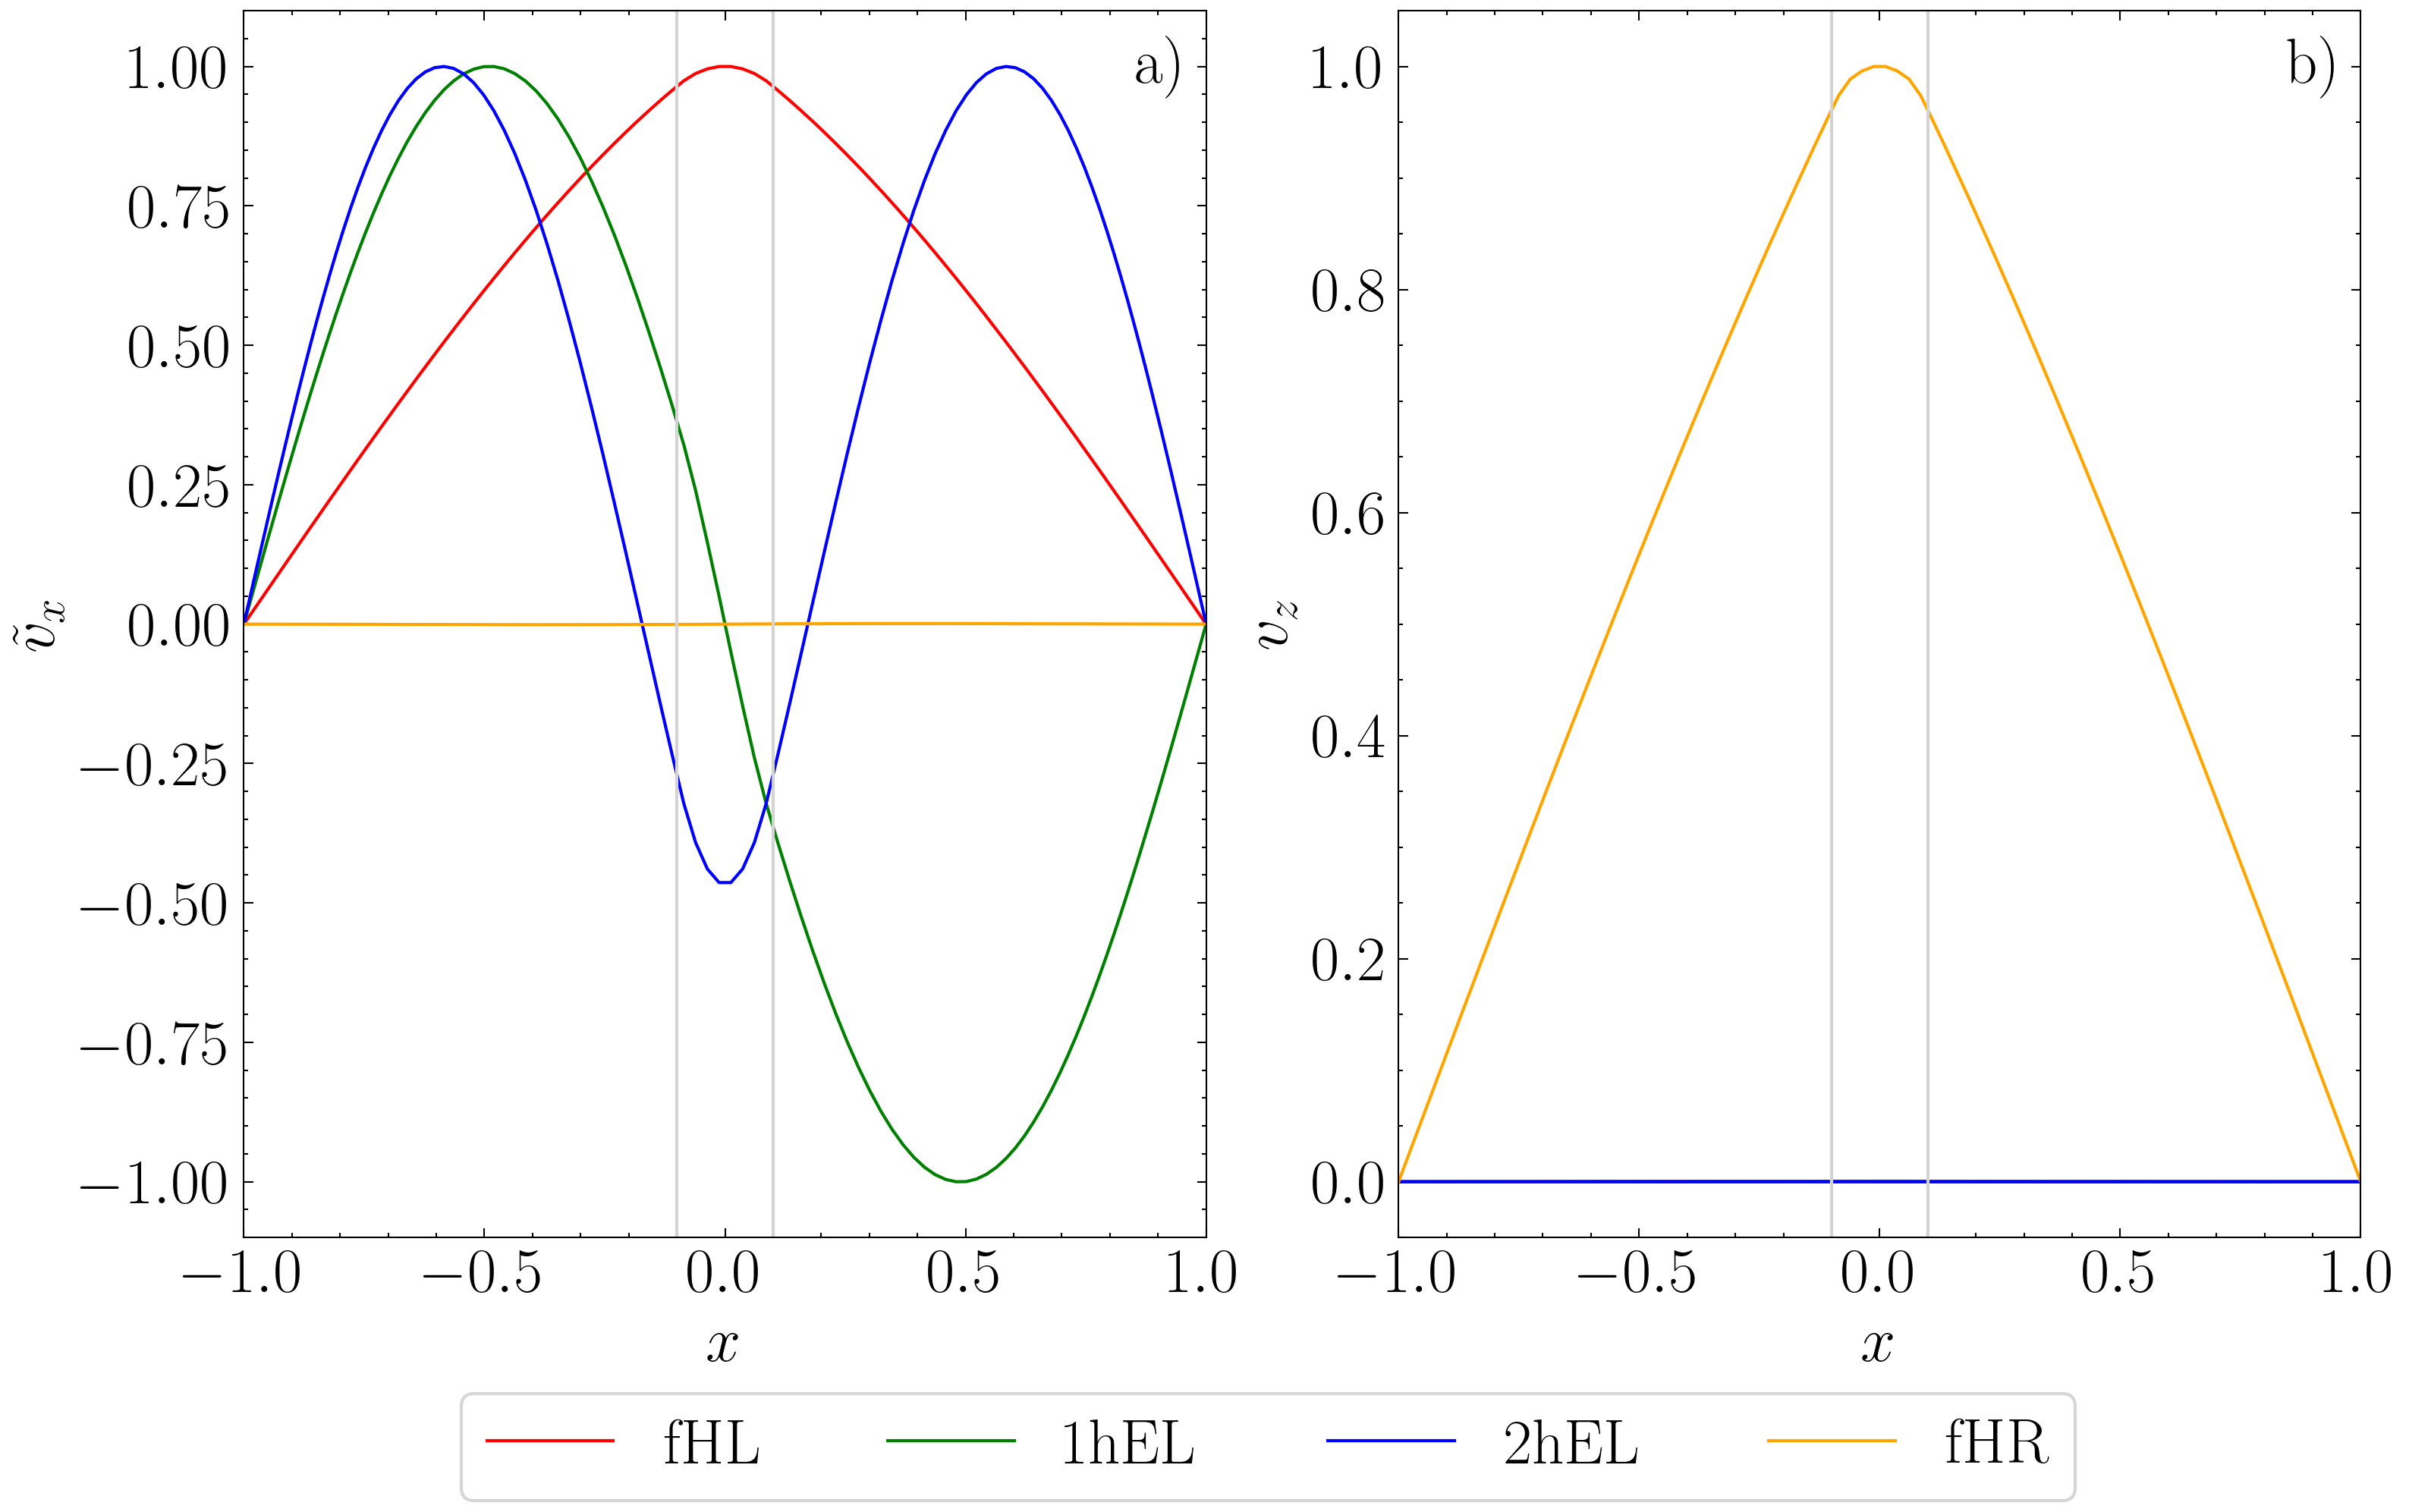
\includegraphics[width=0.95\textwidth]{Figures_F&S_modes/Autofuncions_reals_individuals.png}
	\caption{Estructura de les autofuncions associades als primers 4 modes per $k_z = 0.01$.}
	\label{fig:autofuncions_reals_individuals}
\end{figure}
\vspace{-10pt}
Cada mode correspon a l'etiqueta i color pertinent de la Fig.~\ref{fig:dd}. 
En aquest cas hi ha dues autofuncions, $\tilde{v}_{x}$ i $v_z$, per a cada mode.
El que més destaca respecte als modes d'Alfvén de la Fig.~\ref{fig:modes_vA} és que les autofuncions es subdivideixen per a cada direcció.
En els tres primers modes predomina el terme de $\tilde{v}_{x}$ i forma la mateixa estructura que els primers tres modes d'Alfvén.
En canvi, en el quart mode es giren les tornes i el mode predominant és el de ${v}_{z}$.
Això indica que les tres primeres solucions corresponen a modes lents mentre que la quarta a un ràpid, en el cas de $k_z = 0.01$.
Per tant, la situació està en acord amb el diagrama de dispersió de la Fig.~\ref{fig:dd}.

Segons aquest, amb un valor de la constant d'acoblament superior a la unitat el quart mode també ha de ser lent.
En la següent subsecció es tracta amb detall l'evolució dels modes segons segons la importància de l'acoblament.
Per aquest motiu no es representen les autofuncions d'altres valors de la constant $k_z$.
%Per qüestions d'espai no es representa aquesta situació, tot i que en la següent subsecció es tracta amb detall l'evolució dels modes segons $k_z$.

%---------------------------------------------------------------------------------------------------------------------------------------------------
% DEMANAR A MONXO SI LI PUC ENXUFAR AQUÍ UNA FIGURA MÉS PER COMPROVAR AIXÒ QUE DIC!
%---------------------------------------------------------------------------------------------------------------------------------------------------


\subsubsection{Evolució de les autofuncions segons $k_z$} \label{subsubsec:autofuncions_kz}
%\subsubsection{Autofuncions per kz variable} \label{subsubsec:autofuncions_kz}
Per apreciar el canvi de comportament es comparen les autofuncions aprop de l'encreuament evitat representat en la Fig.~\ref{fig:dd_avoided_crossing}.
Llavors es representa l'estructura dels modes entorn al valor de la constant d'acoblament de $k_z \sim 1$.
\begin{figure}[H]
	\centering
	%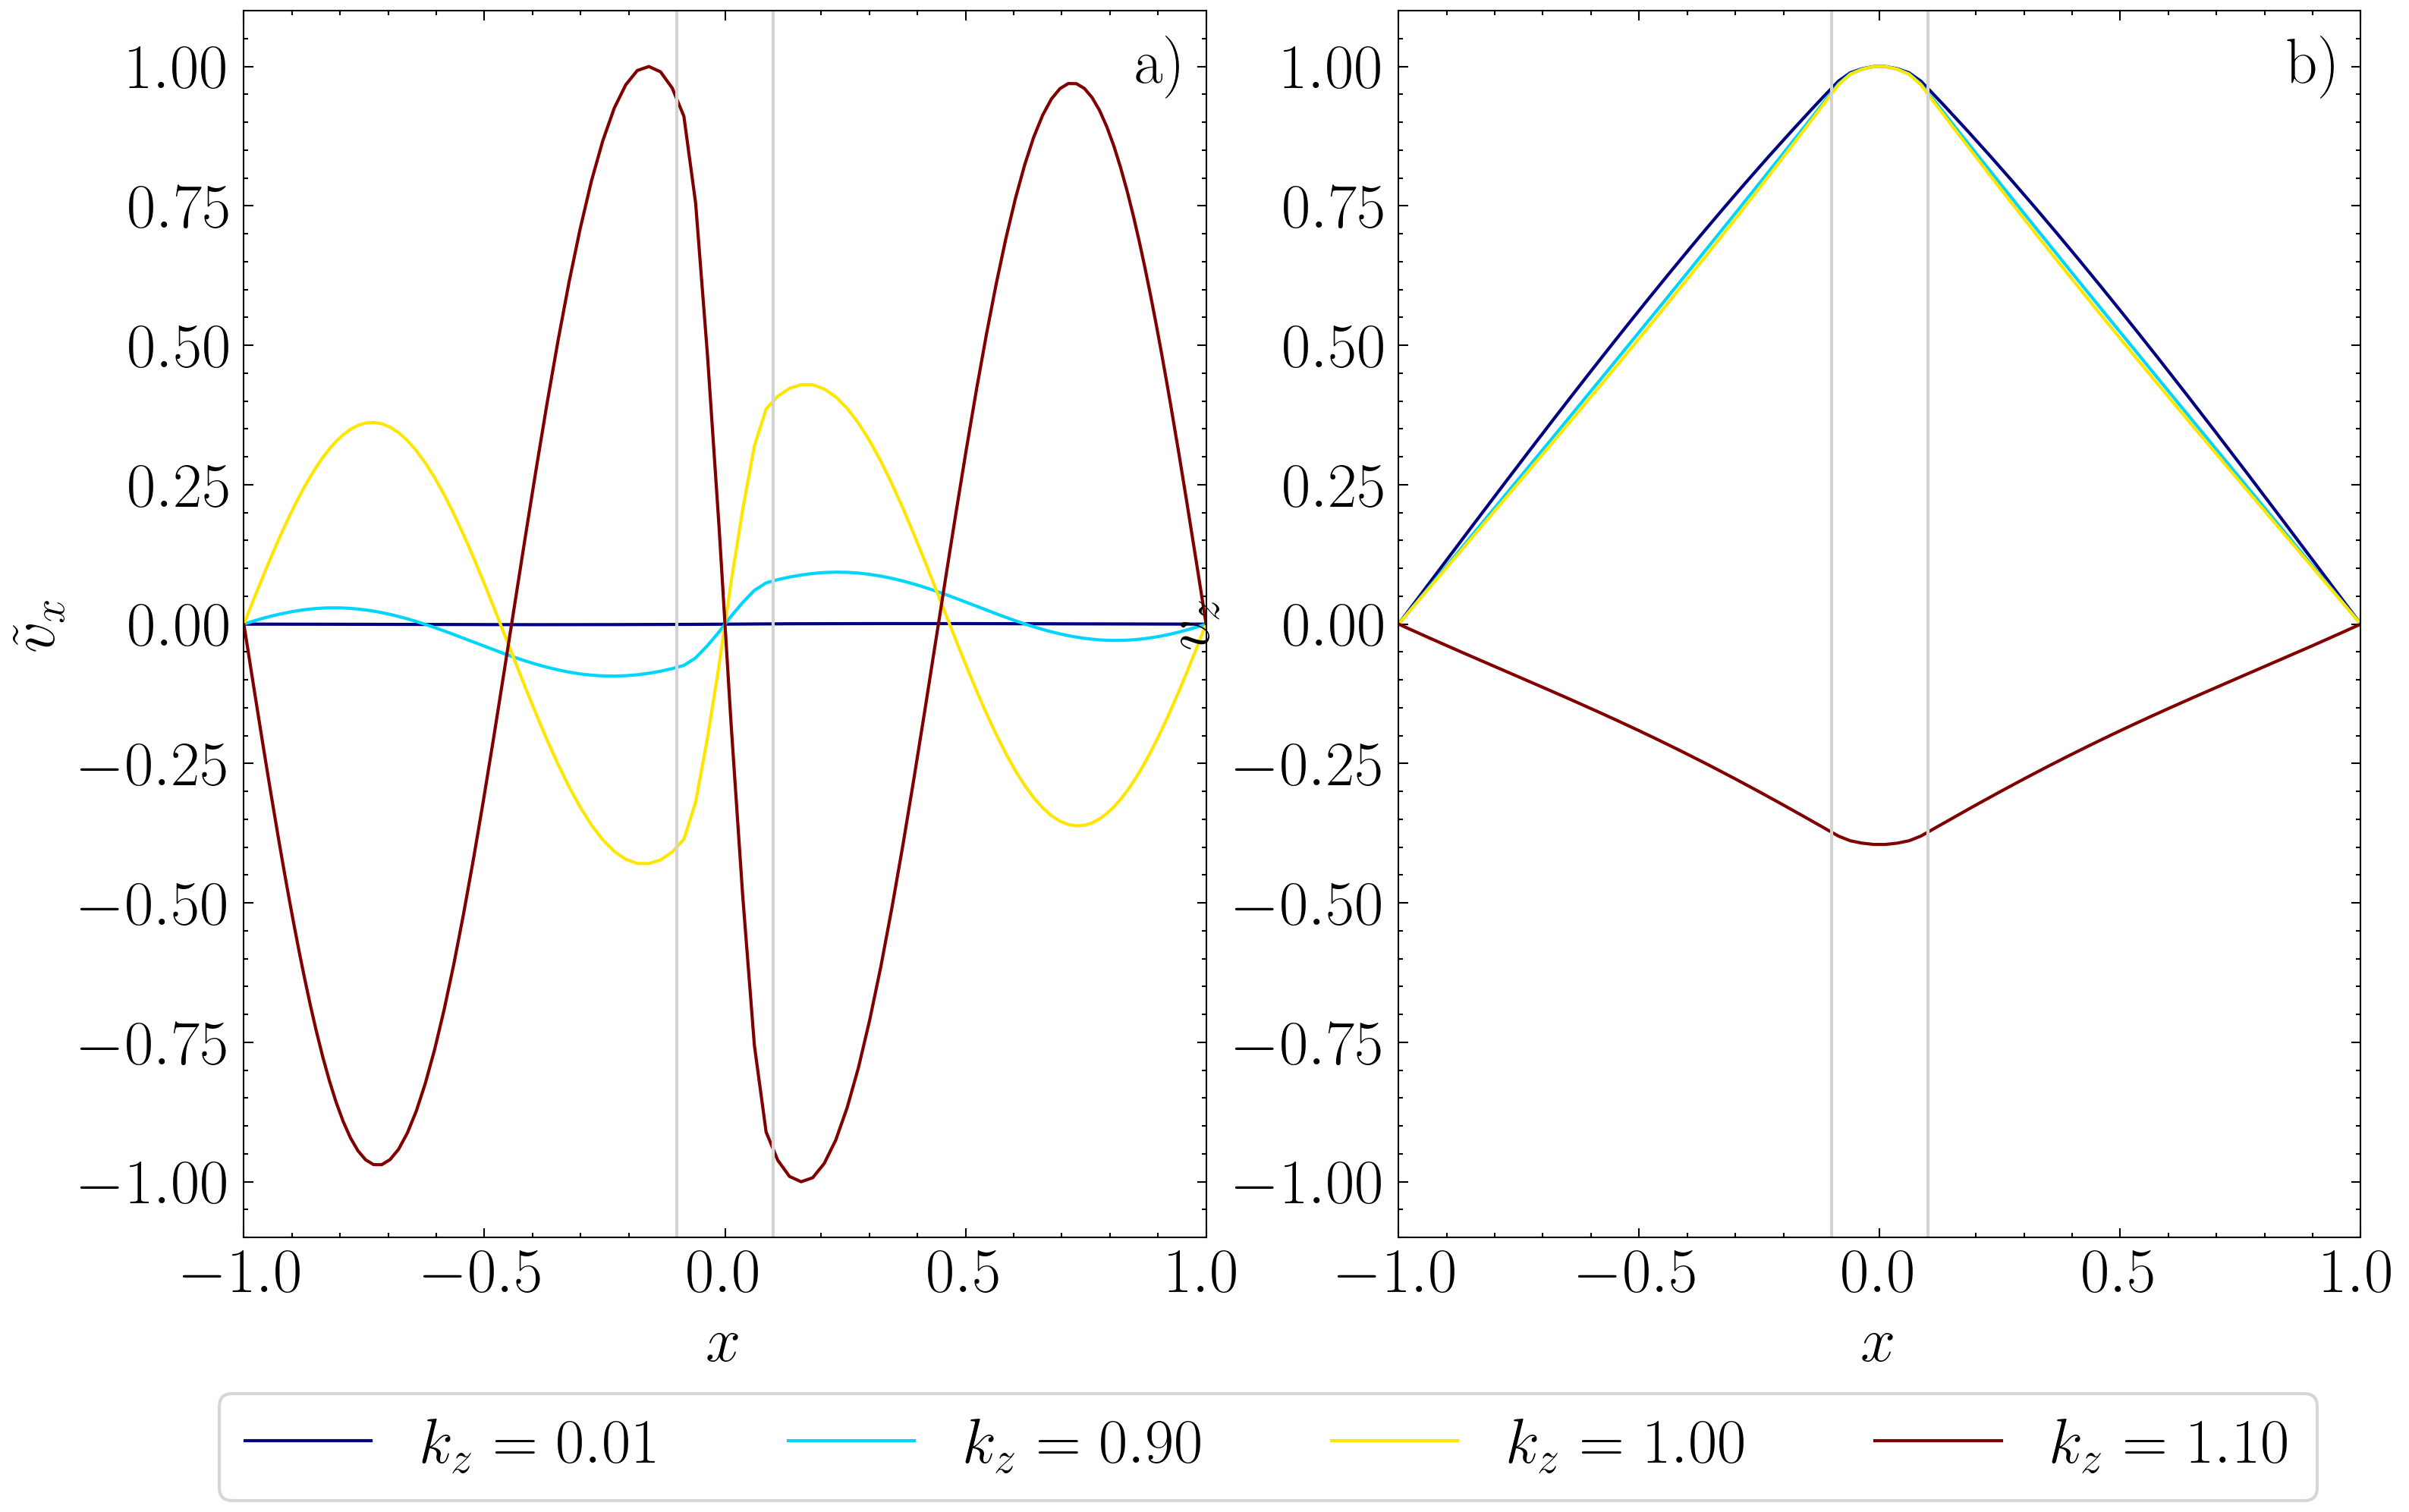
\includegraphics[width=0.95\textwidth]{Figures_F&S_modes/Autofuncions_anticreuament.png}
	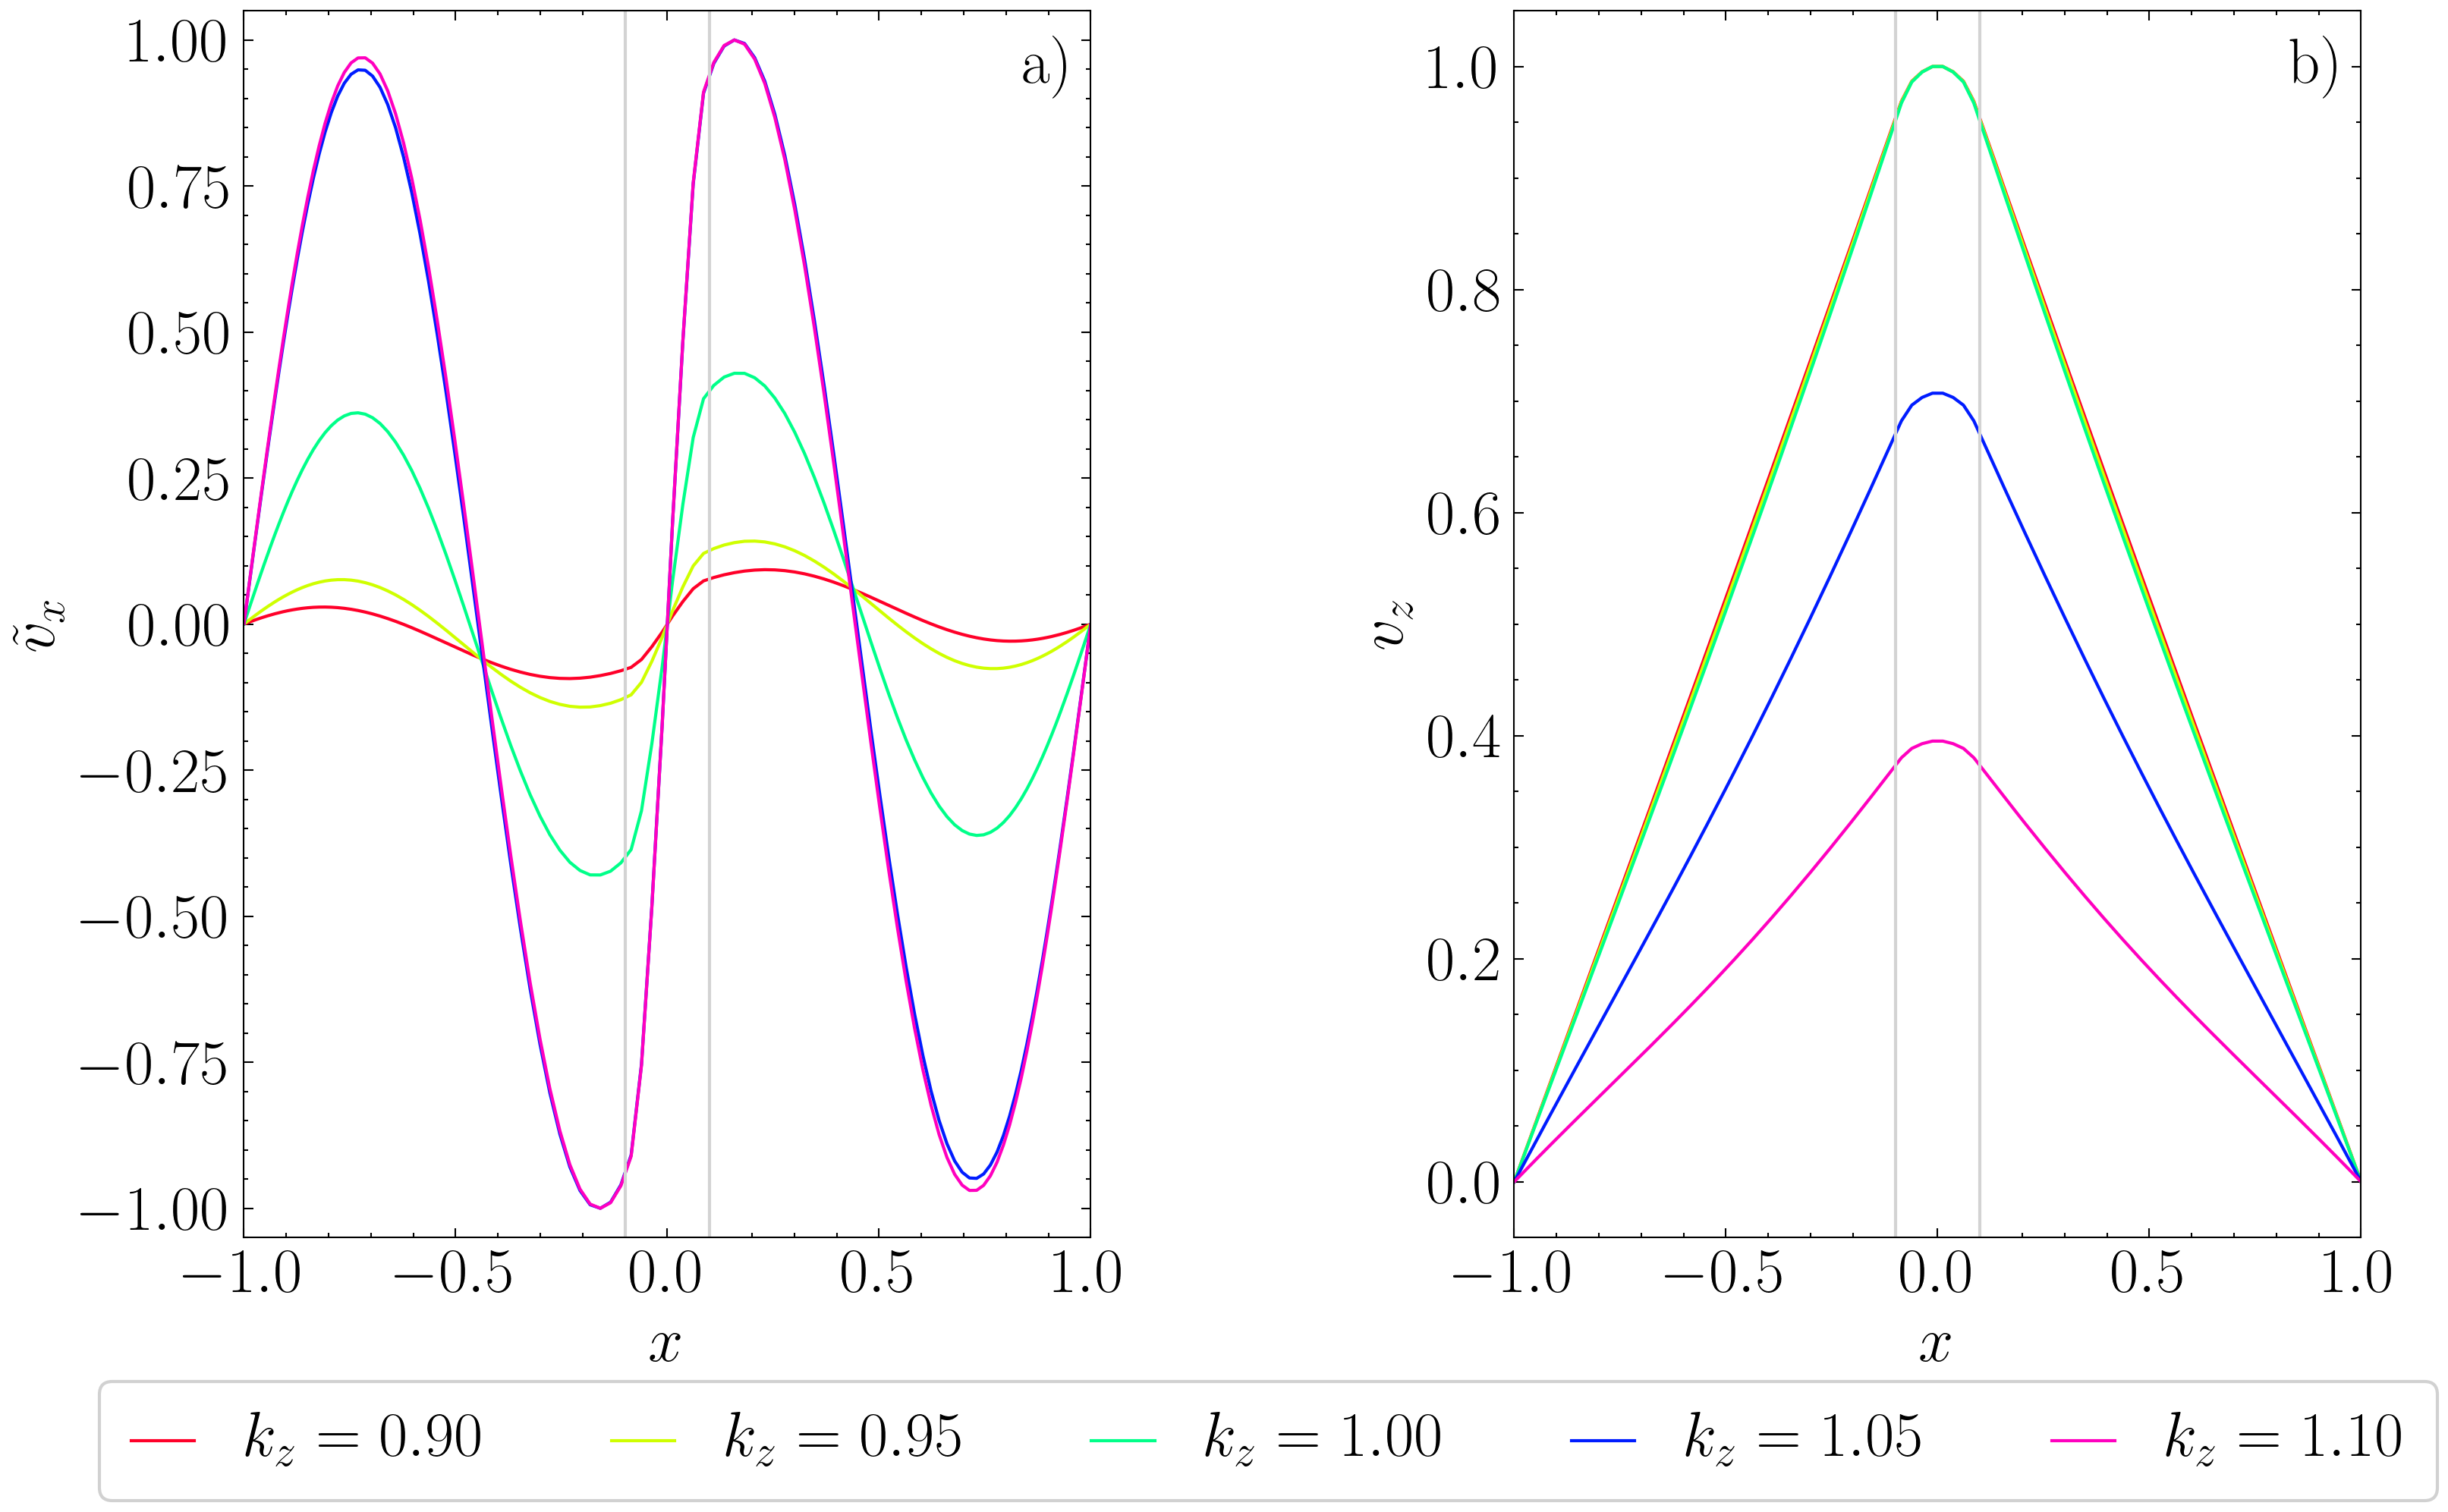
\includegraphics[width=0.95\textwidth]{Figures_F&S_modes/Evolució_autofuncions_n_4_subplots.png}
	\caption{Evolució de les autofuncions del mode fHR en el primer encreuament evitat.}
	\label{fig:autofuncions_anticreuament}
\end{figure}
\vspace{-10pt}
En aquest cas es veu el canvi de dominància d'un mode, $v_z$, enfront a l'altre, $\tilde{v}_{x}$.

Per $k_z = 0.90$ el mode representat en vermell encara és completament dominat per la velocitat en direcció paral·lela al vector d'ona, $v_z$.
En canvi, així com augmenta la constant d'acoblament aquesta, $v_z$, minva i la velocitat normal, $\tilde{v}_{x}$, creix,
segons amb la normalització explicada amb anterioritat.

Finalment, en $k_z = 1.10$ el mode representat en rosa evidencia que la velocitat perpendicular al vector d'ona, $\tilde{v}_{x}$, és major que la paral·lela, $v_z$.
Per tant, s'ha duit a terme un intercanvi de comportament dominant en el mode normal,
així com s'havia predit just abans de començar la \hyperref[subsubsec:autofuncions_kz]{Subsec.~5.2.1}.
%així com s'havia predit en el final de la \hyperref[subsec:resultats_modes_r_i_l]{Subsec.~5.2}.


Per acabar s'estudia l'evolució dels dos modes fonamentals híbrids, per separat,
en funció del valor de l'acoblament en un rang ampli, després de cada encreuament evitat.

Inicialment s'analitza el mode híbrid lent, fHL, en vermell en la relació de dispersió de la Fig.~\ref{fig:dd}.
\begin{figure}[H]
	\centering
	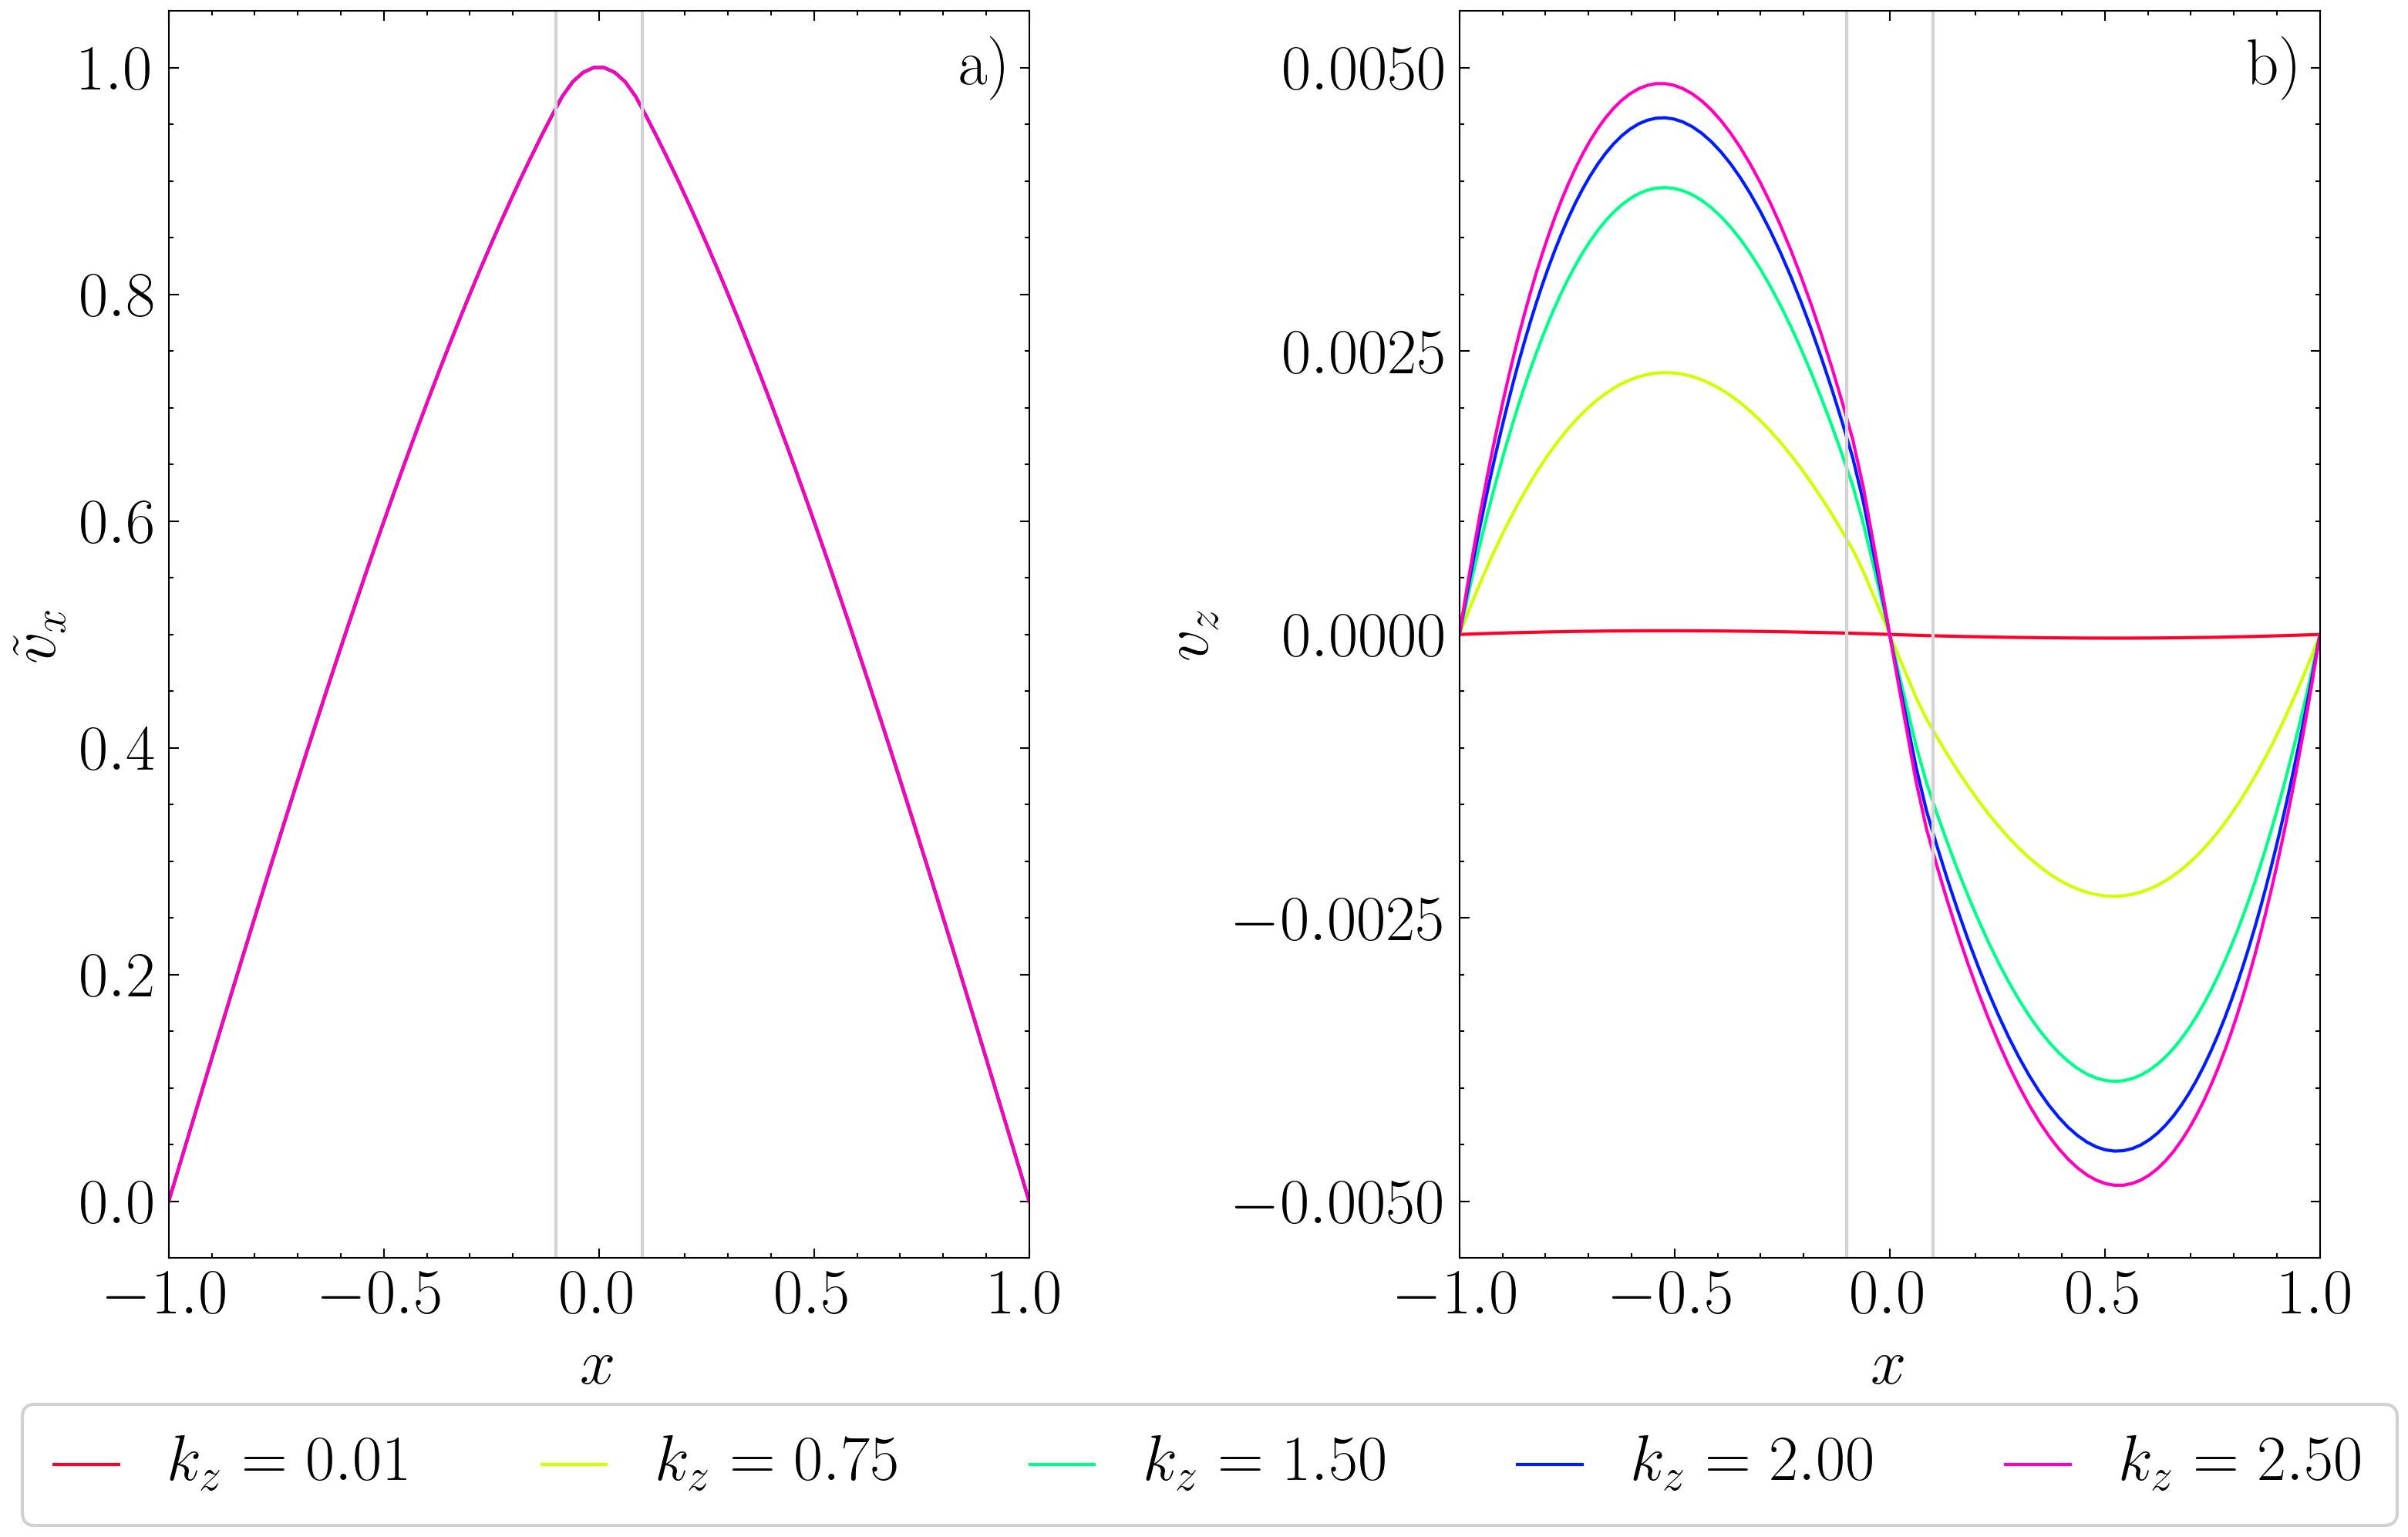
\includegraphics[width=0.95\textwidth]{Figures_F&S_modes/Evolució_autofuncions_fHL_subplots.png}
	\caption{Evolució de les autofuncions del mode fHL segons els encreuaments evitats.}
	\label{fig:fHL}
\end{figure}
\vspace{-10pt}
Les autofuncions són pràcticament invariants, independents de la constant d'acoblament.
Aquest fet és d'esperar ja que en la relació de dispersió el mode és lent, constant, i no es troba amb cap ràpid.
En conseqüència, les autofuncions es solapen atès que són pràcticament idèntiques.
Amb una gran ampliació de la Fig.~\ref{fig:fHL}a en el màxim es pot veure, tot i que es perd la forma del mode de $\tilde{v}_{x}$.

En canvi, l'ampliació és necessària per a l'estudi de l'autofunció minoritària, en aquest cas $v_z$.
El mode és de paritat oposada a l'autofunció dominant, $\tilde{v}_{x}$, que està en estat fonamental, f.
Llavors la minoritària es troba en el primer estat harmònic, 1h.

El major màxim d'aquesta és de l'ordre de $\sim 0.005$ respecte al major màxim de l'altra autofunció dominant.
És per aquest motiu que es requereix de l'eixamplament,
degut a que si es representa a la mateixa escala es perd la informació i sembla una línia recta com en el cas de la Fig.~\ref{fig:autofuncions_reals_individuals}b.
De fet, això mateix passa amb l'autofunció vermella en la pròpia Fig.~\ref{fig:fHL}b,
el mode minoritari és tan inferior al majoritari en valors de $k_z$ baixos, que el cas de $k_z = 0.01$ el mode sembla constant,
tot i que té la mateixa estructura, 1h, que la resta de casos representats.
D'aquesta manera es reflecteix la gran importància de la constant d'acoblament.
Quan és nul·la els modes estan desacoblats i es recupera el cas d'Alfvén, com prediuen les Eqs.~(\ref{eq.3.32}) i (\ref{eq.3.33}).

El segon cas estudiat és el mode híbrid ràpid, fHR, en groc en la relació de dispersió de la Fig.~\ref{fig:dd}.
Tenint en compte que es tracta d'un mode ràpid el seu autovalor, $\omega$, creix de manera parabòl·lica respecte a la constant d'acoblament, $k_z$.
Llavors s'espera que les autofuncions es veguin modificades i reflecteixin l'evolució de l'autovalor.
\begin{figure}[H]
	\centering
	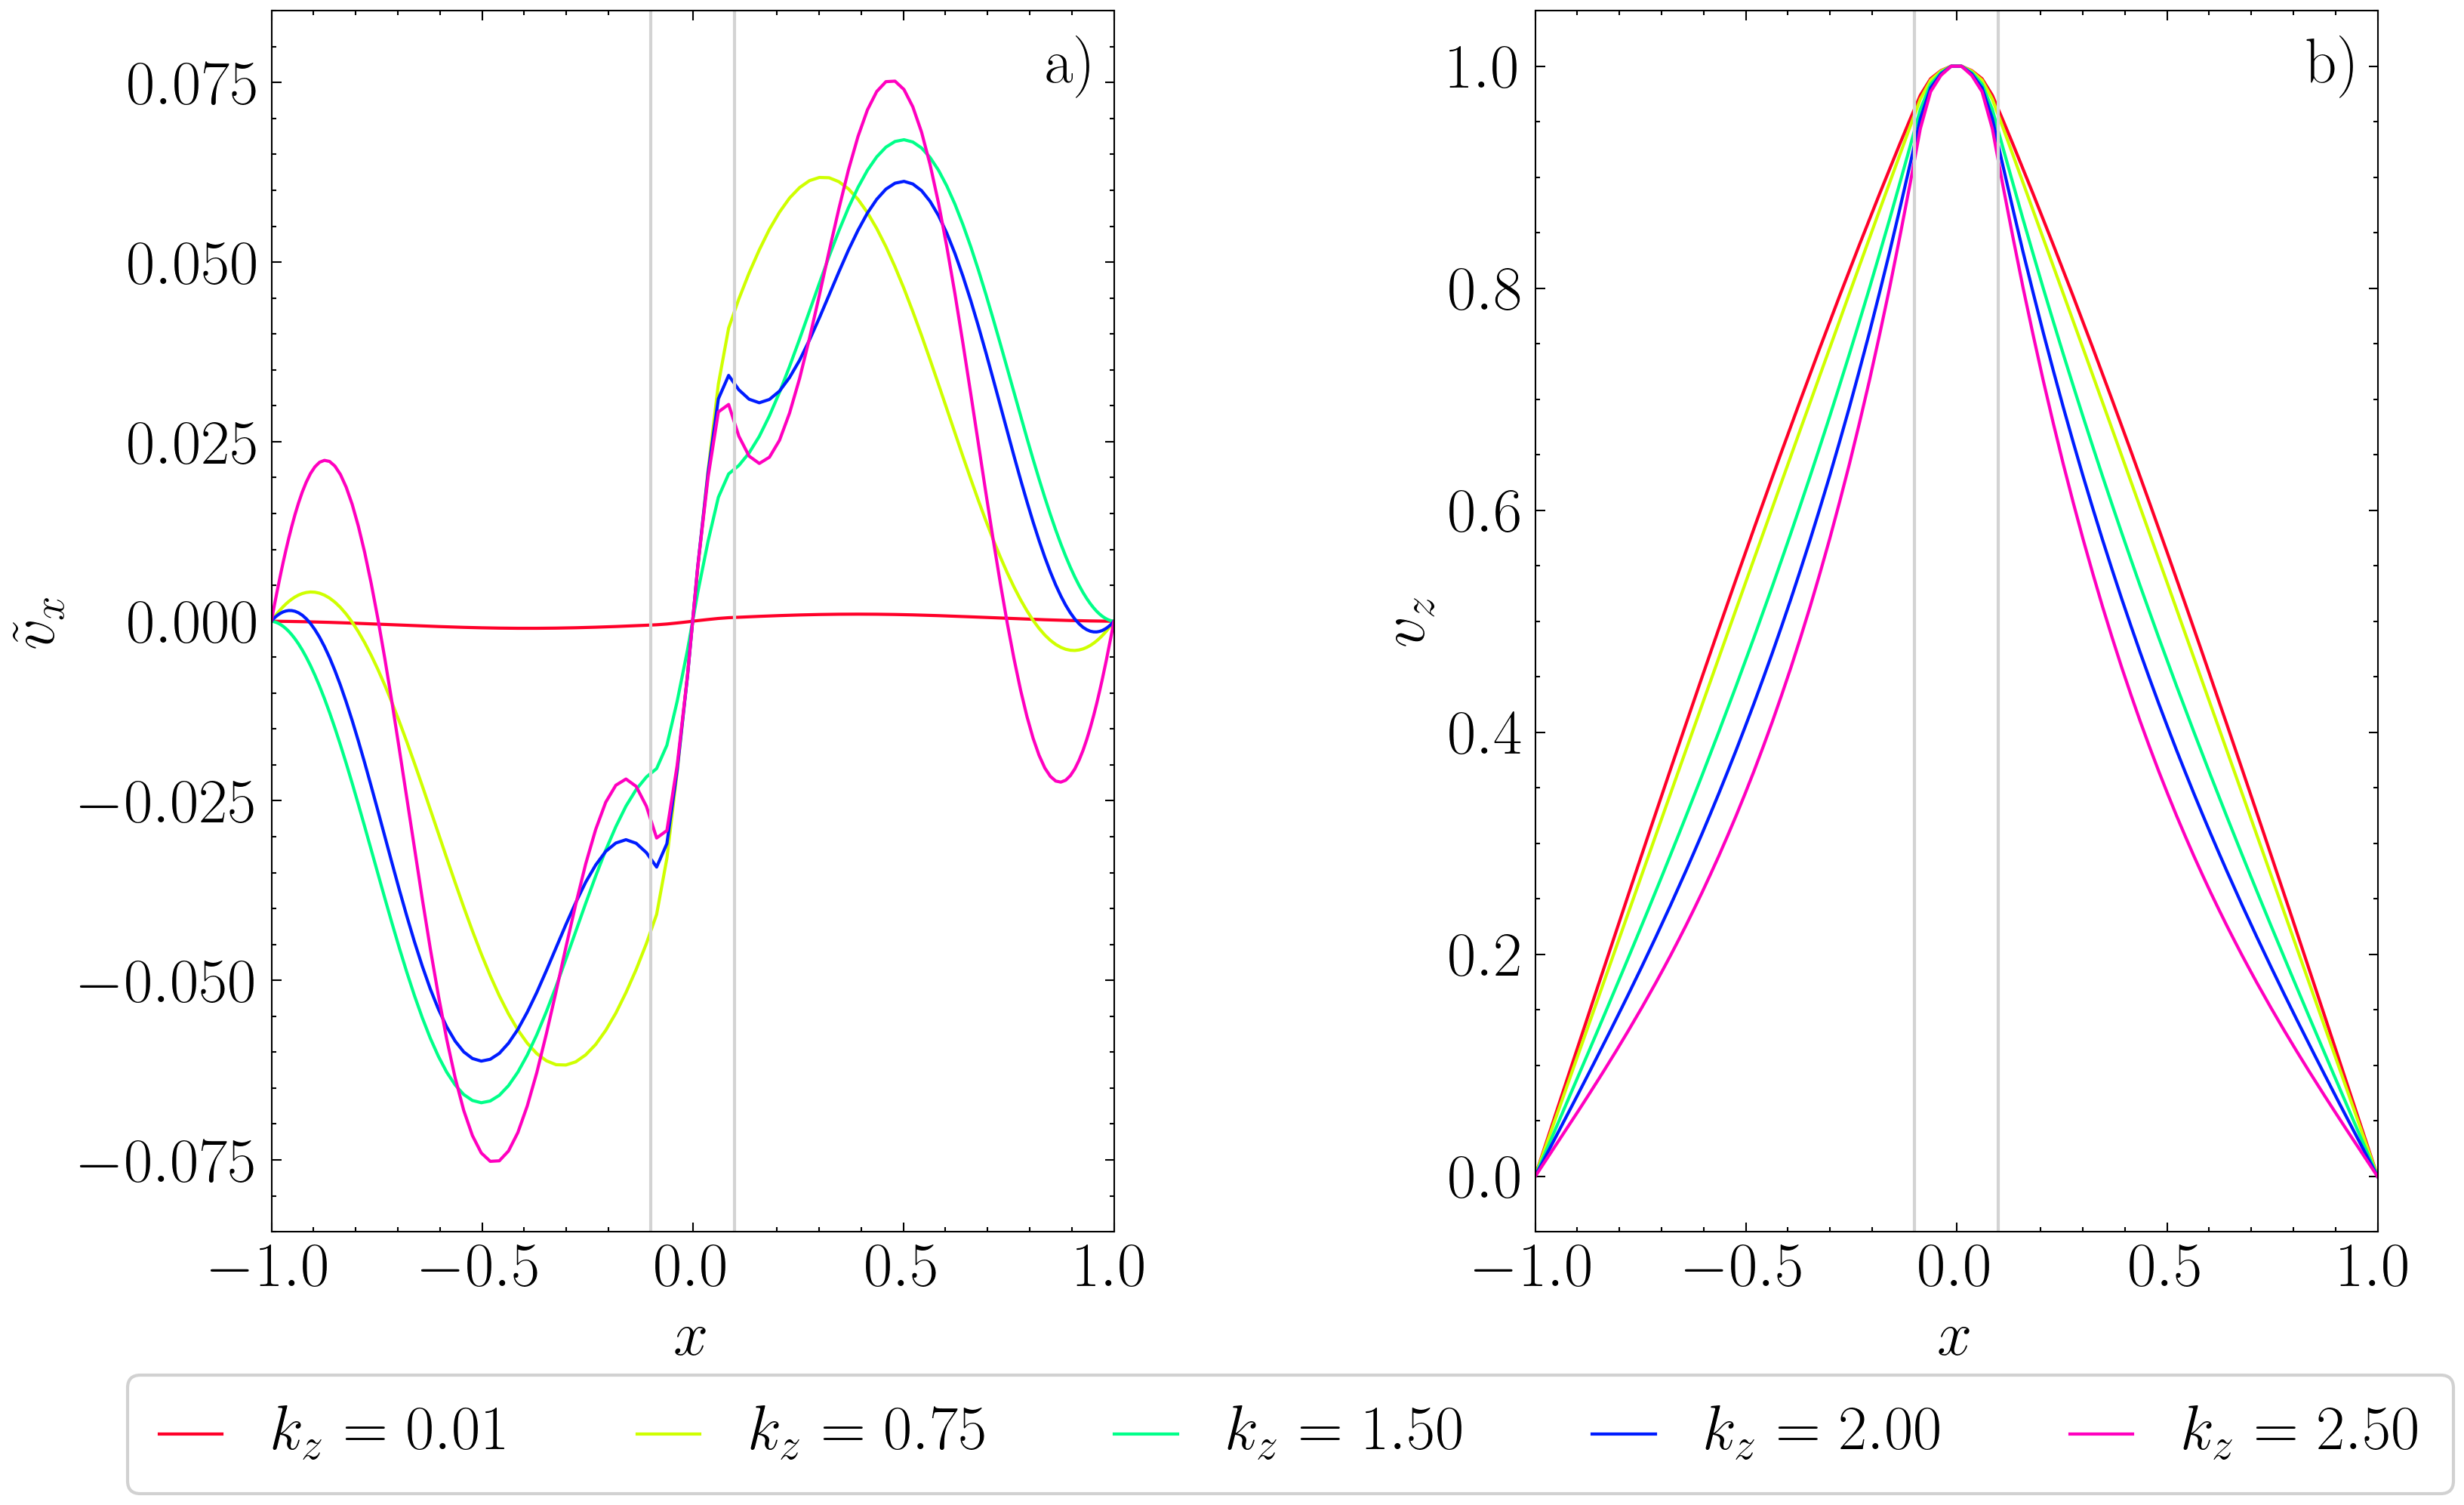
\includegraphics[width=0.95\textwidth]{Figures_F&S_modes/Evolució_autofuncions_fHR_subplots.png}
	\caption{Evolució de les autofuncions del mode fHR segons els encreuaments evitats.}
	\label{fig:fHR}
\end{figure}
\vspace{-10pt}
Efectivament en aquest cas les autofuncions sí pateixen un canvi estructural degut al canvi de $k_z$.

El que més destaca és l'evolució de les autofuncions minoritàries, $\tilde{v}_{x}$.
Per començar, els màxims dels modes en sí creixen a major acoblament, com en el cas anterior.
Cada vegada que es duu a terme un encreuament evitat, els modes dels minoritaris retenen la longitud d'ona del mode lent amb el que han evitat creuar-se.
És per aquest motiu que l'estructura varia considerablement a cada autofunció representada, ja que aquesta s'ha calculat després d'un nou encreuament evitat.
D'aquesta manera, la longitud d'ona del mode decreix a mesura que l'acoblament augmenta, ja que són inversaments proporcionals.

En aquest cas es pot apreciar també com amb poc acoblament, $k_z = 0.01$,
corba vermella, la dominància del mode $v_z$ és encara major precisament perque els modes es troben poc lligats.
A més, s'intueix que es tracta del mateix mode, 3h, que els altres amb un acomblament major,
ja que creua l'eix de les abscisses tres vegades, com la resta de corbes.
A causa de l'escala que pràcticament sembla una recta, tot i que amb una fina mirada s'aprecia que no ho és en cap cas.

El major màxim de les autofuncions minoritàries és $\sim 0.075$,
unes 15 vegades major que el major màxim de les autofuncions minoritàries del primer mode híbrid lent, fHL, de la Fig.\ref{fig:fHL}b.
A més, els dos màxims de les minoritàries té lloc en el cas de major acoblament, amb $k_z = 2.5$.
Llavors es dedueix que la lligadura té un efecte major en els modes ràpids que en els lents.
En els cas de $k_z = 0.75$ la diferència és encara major ja que el màxim del minoritari del mode fHL, $v_z$, és de $\sim 0.0025$,
mentre que el del minoritari del mode fHR, $\tilde{v}_{x}$, és de $\sim 0.06$, unes 24 vegades major.
Definitivament l'acoblament té una major influència en l'estructura dels modes ràpids que en els lents, tot i que no és constant.

Com que es tracta d'un mode ràpid els modes dominants són els de $v_z$. Aquests conserven l'estructura bàsica de mode fonamental, f,
i presenten lleugeres modificacions així com augmenta $k_z$ a causa d'un major acoblament amb les autofuncions minoritàries, $\tilde{v}_{x}$.
El seu comportament es veu alterat com a un estrenyiment de la campana que conforma el mode fonamental a mesura que l'acoblament creix.

L'etiqueta de fonamental, f, en els modes fHL i fHR es deu a l'estructura de l'autofunció dominant del mode corresponent.
Es comprova en els dos casos que les autofuncions presenten una paritat oposada, llavors els modes minoritaris són sempre harmònics senars.
%, 1h i 3h respectivament.